\documentclass[12pt,a4paper]{report}
%\documentclass[12pt,twoside,a4paper]{report}

\usepackage[latin1]{inputenc}
\usepackage[english]{babel}
\usepackage{enumerate}
\usepackage{amsmath}
\usepackage{amssymb}
\usepackage{amsthm}
\usepackage{latexsym}
\usepackage{makeidx}
\usepackage[dvips]{graphicx}
%\usepackage{showidx}
\usepackage[retainorgcmds]{IEEEtrantools}

\makeindex

% --------------------------------------------------------------------- Symbols
\renewcommand{\phi}{\varphi}
\newcommand{\Cayley}{\Psi}
\newcommand{\ModCayley}{\Phi}

% ------------------------------------------------------------------------ Sets
\newcommand{\N}{\mathbb{N}}
\newcommand{\R}{\mathbb{R}}
\newcommand{\Q}{\mathbb{Q}}
\newcommand{\Irrat}{\mathbb{I}}
\newcommand{\Rplus}{\R^{+}}
\newcommand{\C}{\mathbb{C}}
\newcommand{\Z}{\mathbb{Z}}
\newcommand{\EC}{\C_{\infty}}
\newcommand{\EQ}{\Q_{\infty}}
%\newcommand{\RS}{\mathcal{S}}
\newcommand{\UnitCirc}{S^{1}}
\newcommand{\UnitSphere}{S_1}
\newcommand{\EU}{\mathcal{H}^\ast}

\newcommand{\Syms}{\Sigma}
\newcommand{\Words}[1]{{#1}^{\star}}
\newcommand{\FunDom}{\mathcal{F}}
\newcommand{\FunSet}{\mathcal{F}^\ast}
\newcommand{\Indisk}{\mathcal{I}}

\newcommand{\presentation}[2]{\left\langle #1 \mid #2 \right\rangle}
\newcommand{\FreeGrp}[1]{{#1}_{\sim}}

\newcommand{\LinGrp}[3]{\operatorname{#1}_{#2}(#3)}

\newcommand{\GLn}[2]{\LinGrp{GL}{#1}{#2}}
\newcommand{\SLn}[2]{\LinGrp{SL}{#1}{#2}}
\newcommand{\PGLn}[2]{\LinGrp{PGL}{#1}{#2}}
\newcommand{\PSLn}[2]{\LinGrp{PSL}{#1}{#2}}

\newcommand{\GL}[1]{\GLn{2}{#1}}
\newcommand{\SL}[1]{\SLn{2}{#1}}
\newcommand{\PGL}[1]{\PGLn{2}{#1}}
\newcommand{\PSL}[1]{\PSLn{2}{#1}}

\newcommand{\Stabilizer}[2]{{#1}_{#2}}

\newcommand{\Center}[1]{\operatorname{Z}(#1)}

\newcommand{\Mat}[3]{{#1}^{#2 \times #3}}
\newcommand{\SqMat}[2]{\Mat{#1}{#2}{#2}}

\newcommand{\ModGrp}{\Gamma}

\newcommand{\setdefsz}[3]{#1\{ #2 \ #1| \ #3 #1\}}
\newcommand{\setdef}[2]{\setdefsz{}{#1}{#2}}

\newcommand{\fundef}[5]{#1 : \left\{
\begin{matrix} 
#2 &\to& #3 \\ 
#4 &\mapsto& #5
\end{matrix}
\right.}

% ------------------------------------------------------------------ References
\newcommand{\Schoeneberg}{Schoeneberg~\cite{schoeneberg1974elliptic}}
\newcommand{\Klein}{Klein/Fricke~\cite{klein1966vorlesungen}}
\newcommand{\Hungerford}{Hungerford~\cite{hungerford1974algebra}}
\newcommand{\Lehner}{Lehner~\cite{lehner1982discontinuous}}

% ---------------------------------------------------------------------- Macros
\newcommand{\todo}[2]{\bigskip\noindent\framebox[\textwidth]{\emph{TODO #1:} #2}\bigskip}

% --------------------------------------------------------------- Abbreviations
\newcommand{\ie}{i.e.\ }
\newcommand{\eg}{e.g.\ }
\newcommand{\resp}{resp.\ }
\newcommand{\Wlog}{W.l.o.g.\ }

% ------------------------------------------------------------------- Functions
\newcommand{\lxor}{\overset{.}{\lor}}

\newcommand{\floor}[1]{\left\lfloor #1 \right\rfloor}
\newcommand{\ceil}[1]{\left\lceil #1 \right\rceil}
\newcommand{\nint}[1]{\operatorname{nint}\left( #1 \right)}
\newcommand{\sgn}[1]{\operatorname{sgn}\left( #1 \right)}

\newcommand{\topcl}[1]{\operatorname{cl}(#1)}

\newcommand{\half}[1]{\frac{#1}{2}}
\newcommand{\reci}[1]{\frac{1}{#1}}

\newcommand{\cfr}[2]{
\begin{array}{c}\multicolumn{1}{c|}{#1}\\
\hline\multicolumn{1}{|c}{#2}\end{array}}

\newcommand{\inv}[1]{{#1}^{-1}}

\newcommand{\moebius}[5]{\frac{#1 #5 + #2}{#3 #5 + #4}}
\newcommand{\mat}[4]{\begin{pmatrix}#1 & #2 \\ #3 & #4\end{pmatrix}}
\newcommand{\smallmat}[4]{\left({}^{#1}_{#3}\ {}^{#2}_{#4}\right)}
\newcommand{\rvec}[2]{\begin{pmatrix}#1 & #2\end{pmatrix}}
\newcommand{\cvec}[2]{\begin{pmatrix}#1 \\ #2\end{pmatrix}}
\newcommand{\transp}[1]{#1^{\textrm{T}}}
\newcommand{\htransp}[1]{#1^{\textrm{H}}}
\newcommand{\id}[1]{\operatorname{id}_{#1}}

\newcommand{\abs}[1]{\left|#1\right|}
\newcommand{\conj}[1]{\overline{#1}}
\renewcommand{\Re}[1]{\operatorname{Re}\left(#1\right)}
\renewcommand{\Im}[1]{\operatorname{Im}\left(#1\right)}

\newcommand{\epo}[1]{e^{#1}}
\newcommand{\ii}{i}

\newcommand{\eucnorm}[1]{\left\| #1 \right\|_2}

% ---------------------------------------------------------------- Environments

\newtheorem{theorem}{Theorem}[chapter]
\newtheorem{corollary}[theorem]{Corollary}
\newtheorem{lemma}[theorem]{Lemma}

\theoremstyle{definition}
\newtheorem{definition}[theorem]{Definition}
\newtheorem{example}[theorem]{Example}

\theoremstyle{remark}
\newtheorem{remark}[theorem]{Remark}


\title{Computer Algebra and Analysis:\\Complex Variables Visualized}
\author{Thomas Ponweiser}
\date{\today}

\begin{document}

\maketitle

\pagestyle{headings}

\tableofcontents

% ------------------------------------------------------- CHAPTER: INTRODUCTION
\chapter{Introduction}

% -------------------------------------------- Section: Algebraic constructions
\section{Groups and basic algebraic constructions}

In this section, we recapitulate some basic algebraic concepts, most important the notions of \emph{free groups} and \emph{free products}, and the construction of a group in terms of \emph{generators} and \emph{relations}. 

\subsection{Free monoids}
\index{Free!monoid}
Let $\Sigma$ be a set of formal symbols, for example $\Sigma = \{a, b, c, \dots\}$. Then, the set of words over the alphabet $\Sigma$ is defined as
\begin{equation}
\label{eqn_SigmaStarDef}
\Words{\Sigma} := \bigcup_{n\ge0} \Sigma^n.
\end{equation}
We will call the elements of $\Words{\Sigma}$ \emph{words}. To make things easier, we will omit the parentheses when notating such a word $w \in \Words{\Sigma}$, e.g. $w = (a,b,b,a) =: abba$. Note, that also the empty tuple, which we will call the \emph{empty word} and denote as $\epsilon$, is an element of $\Words{\Sigma}$. It is now just natural to define a binary operation $\cdot$ on $\Words{\Sigma}$ which is given by concatenation of words:
\begin{equation*}
w_1 \cdot w_2 = w_1 w_2, \quad w_1, w_2 \in \Words{\Sigma}.
\end{equation*}
Obviously, $\Words{\Sigma}$ is closed under this operation and $\epsilon$ is a the neutral element. Thus $\Words{\Sigma}$ together with the operation $\cdot$ forms a monoid. Note, that in the exceptional case, when $\Sigma = \emptyset$ and thus $\Words{\Sigma} = \{\epsilon\}$, we obtain the trivial monoid by this construction. 

\begin{definition}
\label{dfn_FreeMonoid}
Let $\Sigma$ be an arbitrary set of symbols (called the alphabet), and $\Words{\Sigma}$ be defined as in (\ref{eqn_SigmaStarDef}). Moreover, denote concatenation of words by $\cdot$ and let $\epsilon$ be the empty word. Then, the algebraic structure $\langle \Words{\Sigma}, \cdot, \epsilon \rangle$ is called the \emph{free monoid over the alphabet $\Sigma$}.
\end{definition} 

\subsection{Free groups}
\index{Free!group}
In a similar fashion, we can construct also a group from any given formal alphabet $\Sigma$. For this purpose we first choose a disjoint copy of $\Sigma$, denoted by $\inv{\Sigma}$, and a bijection $f : \Sigma \to \inv{\Sigma}$. We can extend this bijection between the sets $\Sigma$ and $\inv{\Sigma}$ to an involution on their union $\overline{\Sigma} := (\Sigma \cup \inv{\Sigma})$ by simply defining $f(f(a)) := a$ for all $a \in \Sigma$. Now we introduce the notation $f(a) =: \inv{a}$ and call $\inv{a}$ the \emph{(formal) inverse} of the symbol $a \in \overline{\Sigma}$.

\index{Reduced form}
Next, we construct the free monoid $\Words{\overline{\Sigma}}$. If $\sigma_1, \sigma_2, \dots, \sigma_n$ are symbols of $\overline{\Sigma}$, then we say the word $\sigma_1 \sigma_2 \dots \sigma_n$ is \emph{reduced}, if and only if no two subsequent symbols of the word are inverse to each other, that is
\begin{equation}
\label{eqn_GrpWordReducedForm}
 \sigma_j \ne \sigma_{j+1}^{-1} \quad \text{for all } 1 \le j < n.
\end{equation}
Clearly, every word $w \in \Words{\overline{\Sigma}}$ can be brought into reduced form by successively ``canceling out'' adjacent inverse symbols until finally a word is obtained, which satisfies (\ref{eqn_GrpWordReducedForm}). We call the result of this procedure the \emph{reduced form of $w$}. Additionally, we define two words $w_1, w_2 \in \Words{\overline{\Sigma}}$ to be \emph{equivalent}, if and only if they have the same reduced form and we write $w_1 \sim w_2$ in this case. It is easy to see that this relation is a congruence relation (i.e. is compatible with word-concatenation)\footnote{Denote the reduced form of a word $w$ as $\phi(w)$. If $w_1 \sim w_2$ and $v_1 \sim v_2$ are given, then we also have $w_1 v_1 \sim w_2 v_2$ because $\phi(w_1) = \phi(w_2) := w$ and $\phi(v_1) = \phi(v_2) := v$ implies $\phi(w_1 v_1) = \phi(w v) = \phi(w_2 v_2)$.} and thus we can consider also the set of equivalence classes $\Words{\overline{\Sigma}}/_{\sim}$ as monoid under the operation of word-concatenation. Obviously the set of reduced words is a representative system for $\Words{\overline{\Sigma}}/_{\sim}$ and we agree to denote an equivalence class $[w]_{\sim}$ simply by the reduced word $w$. $\Words{\overline{\Sigma}}/_{\sim}$ is not just a monoid, but in fact a group, as the inverse of a word $\sigma_1 \sigma_2 \dots \sigma_{n-1} \sigma_n$ is trivially given by $\sigma_n^{-1} \sigma_{n-1}^{-1} \dots \sigma_2^{-1} \sigma_1^{-1}$. 
\begin{definition}
\label{dfn_FreeGroup}
Let $\Sigma$ be an arbitrary set of formal symbols and define $\overline{\Sigma} := \Sigma \cup \inv{\Sigma}$ as above. On the free monoid $\Words{\overline{\Sigma}}$ define an equivalence relation $\sim$ by identifying words with same reduced form. Then, the algebraic structure $\langle \Words{\overline{\Sigma}}/_{\sim}, \cdot, \epsilon \rangle$ is called the \emph{free group over the alphabet $\Sigma$}.
\end{definition}
\begin{remark}
In the exceptional case, when $\Sigma = \emptyset$  we obtain the trivial group by this construction\footnote{If $\Sigma = \emptyset$ then we can also choose $\inv{\Sigma} = \emptyset$ ($\Sigma$ and $\inv{\Sigma}$ are then disjoint as required). It follows that also $\overline{\Sigma}$ is empty and we end up with the trivial monoid $\{\epsilon\}$, which is in the same time the trivial group.}.
\end{remark}


% --------------------------------------------- Section: M�bius transformations
\section{M�bius transformations}

In the following we define the group of M�bius transformations and collect some useful basic properties.

\begin{definition}
\label{dfn_MoebiusTransform}
\index{Mobius transformation@M�bius transformation}
A non-constant rational function $\phi \in \C(z)$ of the form 
\begin{equation*}
\phi(z) = \moebius{a}{b}{c}{d}{z},\quad a, b, c, d \in \C,\quad ad - bc \ne 0
\end{equation*}
is called \emph{M�bius transformation}.
\end{definition}

\begin{remark}
The condition $ad - bc \ne 0$ just ensures that $\phi$ is in fact non-constant.
\end{remark}

\begin{theorem}
\label{thm_MoebiusGroup}
The set of M�bius transformations forms a group under the action of function composition and can be identified with the projective general linear group $\PGL{\C}$ or the projective special linear group $\PSL{\C}$.
\end{theorem}
\begin{proof}
Let $\phi$ and $\psi$ be M�bius transformations with
\begin{equation*}
\phi(z) = \moebius{a}{b}{c}{d}{z},\quad \psi(z) = \moebius{e}{f}{g}{h}{z}.
\end{equation*}

First, we make the trivial observation, that composing those two transformations again yields a rational function of the desired form:
\begin{equation}
\label{eqn_MoebiusComposition}
\phi \circ \psi(z) 
 = \moebius{a}{b}{c}{d}{\moebius{e}{f}{g}{h}{z}} 
 = \frac{aez + af + bgz + bh}{cez + cf + dgz + dh} 
 = \moebius{(ae + bg)}{(af + bh)}{(ce + dg)}{(cf + dh)}{z}
\end{equation}

Having a closer look on the resulting coefficients one might notice that they relate to the following matrix product:
\begin{equation}
\label{eqn_MatrixProduct}
\mat{a}{b}{c}{d} \cdot \mat{e}{f}{g}{h} 
 = \mat{ae + bg}{af + bh}{ce + dg}{cf + dh}
\end{equation}

This motivates the definition of a mapping $\pi$ between matrices in $\GL{\C}$ and M�bius transformations:
\begin{equation}
\label{eqn_homPi}
\pi: \mat{a}{b}{c}{d} \mapsto \left(z \mapsto \moebius{a}{b}{c}{d}{z}\right)
\end{equation}
Note, that the domain of $\pi$ is $\GL{\C}$, \ie the set of 2-by-2 matrices with nonzero determinant. This is perfectly consistent with the condition $ad - bc \ne 0$ we have for M�bius transformations. For this reason, $\pi$ is a well-defined function from $\GL{\C}$ to the set of M�bius transformations.

But $\pi$ is not just a function, it is in fact a homomorphism, as we have seen in (\ref{eqn_MoebiusComposition}) and (\ref{eqn_MatrixProduct}). Trivially, $\pi$ is also surjective, which carries over the group structure of $\GL{\C}$ to the set of M�bius transformations. The kernel of $\pi$ comprises of all multiples of the identity matrix. Therefore, by the first isomorphism theorem the group of M�bius transformations is isomorphic to $\GL{\C}/\ker{\pi} \cong \PGL{\C}$ and we have seen in Example \ref{ex_ProjAndGenLinGrp} that $\PGL{\C} \cong \PSL{\C}$.
\end{proof}

\begin{remark}
We note that the nature of M�bius transformations is threefold: Firstly, as in Definition~\ref{dfn_MoebiusTransform}, we can regard a M�bius transformation $\phi$ as purely algebraic object, namely as rational function, \ie the (formal) quotient of two polynomials in $\C[z]$:
\begin{equation*}
\phi_{\text{alg}} = \moebius{a}{b}{c}{d}{z} \in \C(z).
\end{equation*} 
Secondly, $\phi$ has a natural interpretation as meromorphic function on the extended complex plane $\EC = \C \cup \{\infty\}$ in the sense of complex analysis:
\begin{equation*}
\phi_{\text{fun}}: \left\{ 
\begin{array}{ccc}
\EC &\to& \EC \\
z  &\mapsto& \moebius{a}{b}{c}{d}{z}
\end{array}
\right.
\end{equation*}
In a more formal context, this correspondence can also be seen the following way: The group of M�bius transformations acts on the set $\EC$ in the sense of Defintion~\ref{dfn_GroupAction} by $\phi_{\text{alg}} z := \phi_{\text{fun}}(z)$. Now, the homomorphism of Theorem~{\ref{thm_GroupActionHom}} is in fact an isomorphism which assigns each M�bius transformation $\phi_{\text{alg}}$ a permutation of the set $\EC$ which is exactly the meromorphic function $\phi_{\text{fun}}$.
Last but not least, we have seen in Theorem~\ref{thm_MoebiusGroup} that we can also regard $\phi$ as equivalence class of matrices:
\begin{equation*}
\phi_{\text{lin}} = \mat{a}{b}{c}{d}_{\sim} \in \PGL{\C}.
\end{equation*}
Whenever there is no danger of confusion, we will from now on switch between these different views on M�bius transformations seamlessly and exploit concepts of algebra, function theory and linear algebra alternately.
\end{remark}

\begin{lemma}
\label{lem_MoebiusGenerators}
The group of M�bius transformations is generated by the following basic types of transformations:

\begin{tabular}{r l l l}
\index{Translation}
\index{Rotation}
\index{Dilation}
\index{Inversion}
$\bullet$ & Translations: & $z \mapsto z + \alpha$         & $\alpha \in \C$ \\
$\bullet$ & Dilations:    & $z \mapsto \rho z$             & $\rho > 0$ \\
$\bullet$ & Rotations:    & $z \mapsto \epo{\ii \theta} z$ & $\theta \in (-\pi,\pi]$ \\
$\bullet$ & Inversion:   & $z \mapsto \reci{z}$           & ~ 
\end{tabular}
\end{lemma}
\begin{proof}
Let $\phi(z) = \moebius{a}{b}{c}{d}{z}$ be an arbitrary M�bius transformation. In the case when $c = 0$, we may further assume w.l.o.g. that $d = 1$ such that the transformation simply writes $\phi(z) = a z + b$. Obviously this is dilation and rotation by the factor $a$ followed by translation by $b$.

Let's consider the more interesting case, when $c \ne 0$. Without restriction we may assume that $c = 1$, such that 
\begin{equation*}
\phi(z) = \moebius{a}{b}{}{d}{z} = a + \frac{b - ad}{z + d}.
\end{equation*}
Also in this case it is easy to see that $\phi$ is composed of translation by $d$, inversion, dilation and rotation by the factor $b - ad$ and a final translation by $a$.
\end{proof}

Now that we have defined the group of M�bius transformations, it is worth to get a better geometric intuition about how these maps act on the complex plane. Lemma \ref{lem_MoebiusGenerators} gives a first insight, as translations, dilations and rotations are quite easy to understand. Also the map $z \mapsto \reci{z}$ has a geometric interpretation, namely as circle inversion followed by a reflection.

\index{Circle inversion}
\index{Inversion}
In 2-dimensional geometry, \emph{circle inversion} with respect to a reference circle with center $C$ and a radius $r$ takes each point $P$ on the plane to a point $P^{\prime}$ which is determined by $CP \cdot CP^{\prime} = r^2$. The image of $C$ is defined to be the point at infinity (and vice versa). Roughly speaking, the inversion turns the circle ``inside out'', \ie points inside the reference circle are bijectively mapped to points outside while rays from the circle center are invariant under the circle inversion.

\todo{15}{Figure for circle inversion}

Coming back to the concrete map $z \mapsto \reci{z}$, it can now be interpreted the following way: Circle inversion with regard to the unit circle $\UnitCirc$ maps each $z \in \C$ to $\frac{z}{\abs{z}^2} = \reci{\conj{z}}$. Then, reflection across the real axis (\ie complex conjugation) takes $\reci{\conj{z}}$ to $\reci{z}$. 

Summing up, all the basic types of M�bius transformations mentioned in Lemma \ref{lem_MoebiusGenerators} have a very direct geometric interpretation. Still, arbitrary M�bius transformations (especially those involving at least one inversion) are hard to describe in a similar geometric and intuitive way. 

Luckily there is another characterization of M�bius transformations which is both, elegant and visually accessible.

% ---------------------------------------- Subsection: Stereographic projection
\subsection{Stereographic projection}

This section is about the great work of Douglas Arnold and Jonathan Rogness, ``M�bius transformations revealed'' \cite{arnold2008mobius}, in which the authors give a characterization of M�bius transformations in terms of stereographic projections and rigid motions of spheres in 3D-space.

\index{Euclidean norm}
In order to introduce stereographic projection, we first have to embed $\C$ into $\R^3$. We do so by using the map 
\begin{equation}
\iota : \left\{\begin{array}{ccc}
\C & \to & \R^3 \\
z  & \mapsto & \left(\Re{z}, \Im{z}, 0\right)
\end{array}\right.,
\end{equation}
which means that we identify the complex plane with the plane $x_3 = 0$ in $\R^3$. Additionally we equip $\R^3$ with the standard Euclidean norm:
\begin{equation}
\eucnorm{x} := \sqrt{x_1^2 + x_2^2 + x_3^2}, \quad x \in \R^3.
\end{equation}

\begin{definition}[Admissible sphere]
\index{Admissible sphere}
A \emph{sphere} with center $c \in \R^3$ and radius $r > 0$ is the set $S := \setdef{x \in \R^3}{\eucnorm{x - c} = r}$. Its \emph{north-pole} is the unique point $n \in S$ with maximal $x_3$-coordinate. A sphere whose north pole lies in the upper half-space $H := \setdef{x \in \R^3}{x_3 > 0}$ is called an \emph{admissible sphere}.
\end{definition}

\begin{definition}[Stereographic projection]
\index{Stereographic projection}
\label{dfn_StereoProject}
Let $S$ be an admissible sphere and $n \in S$ be its north pole. If $x \in S \setminus \{n\}$, then denote by $L_{x,n}$ the unique line joining $x$ with $n$ and let $y$ be the intersection point of $L_{x,n}$ with the plane $\iota(\C)$. Now, \emph{stereographic projection} with regard to $S$ is the map $P_S : S \to \EC$ defined as $P_S(x) := \inv{\iota}(y)$ for $x \ne n$ and $P_S(n) := \infty$.
\end{definition}

\begin{remark}
\label{rem_RiemannSphere}
\index{Riemann sphere}
Stereographic projection with regard to any admissible sphere $S \subseteq \R^3$ maps $S$ bijectively to $\EC$. Of course the most natural choice for $S$ in this context is the unit sphere $\UnitSphere := \setdef{x \in \R^3}{\eucnorm{x} = 1}$, having the advantage that stereographic projection follows the simple formula
\begin{equation}
\label{eqn_StdStereoProj}
P_{\UnitSphere}:
\begin{pmatrix} x_1 \\ x_2 \\ x_3 \end{pmatrix} 
\mapsto \frac{x_1 + \\i x_2}{1 - x_3}.
\end{equation}
Also reverse stereographic projection can be done easily using the unit sphere:
\begin{equation}
\label{eqn_RevStdStereoProj}
P_{\UnitSphere}^{-1}: z \mapsto 
\reci{\abs{z}^2 + 1} 
\begin{pmatrix}2 \Re{z} \\ 2 \Im{z} \\ \abs{z}^2 - 1\end{pmatrix}.
\end{equation}
By pointwise identifying $\EC$ with $S_1$ using the above two mappings, we obtain the $\emph{Riemann sphere}$ model of the extended complex plane. One of its benefits is that certain functions $\EC \to \EC$ can be interpreted nicely as simple rotations of the Riemann sphere.
\end{remark}

\begin{figure}
\centering
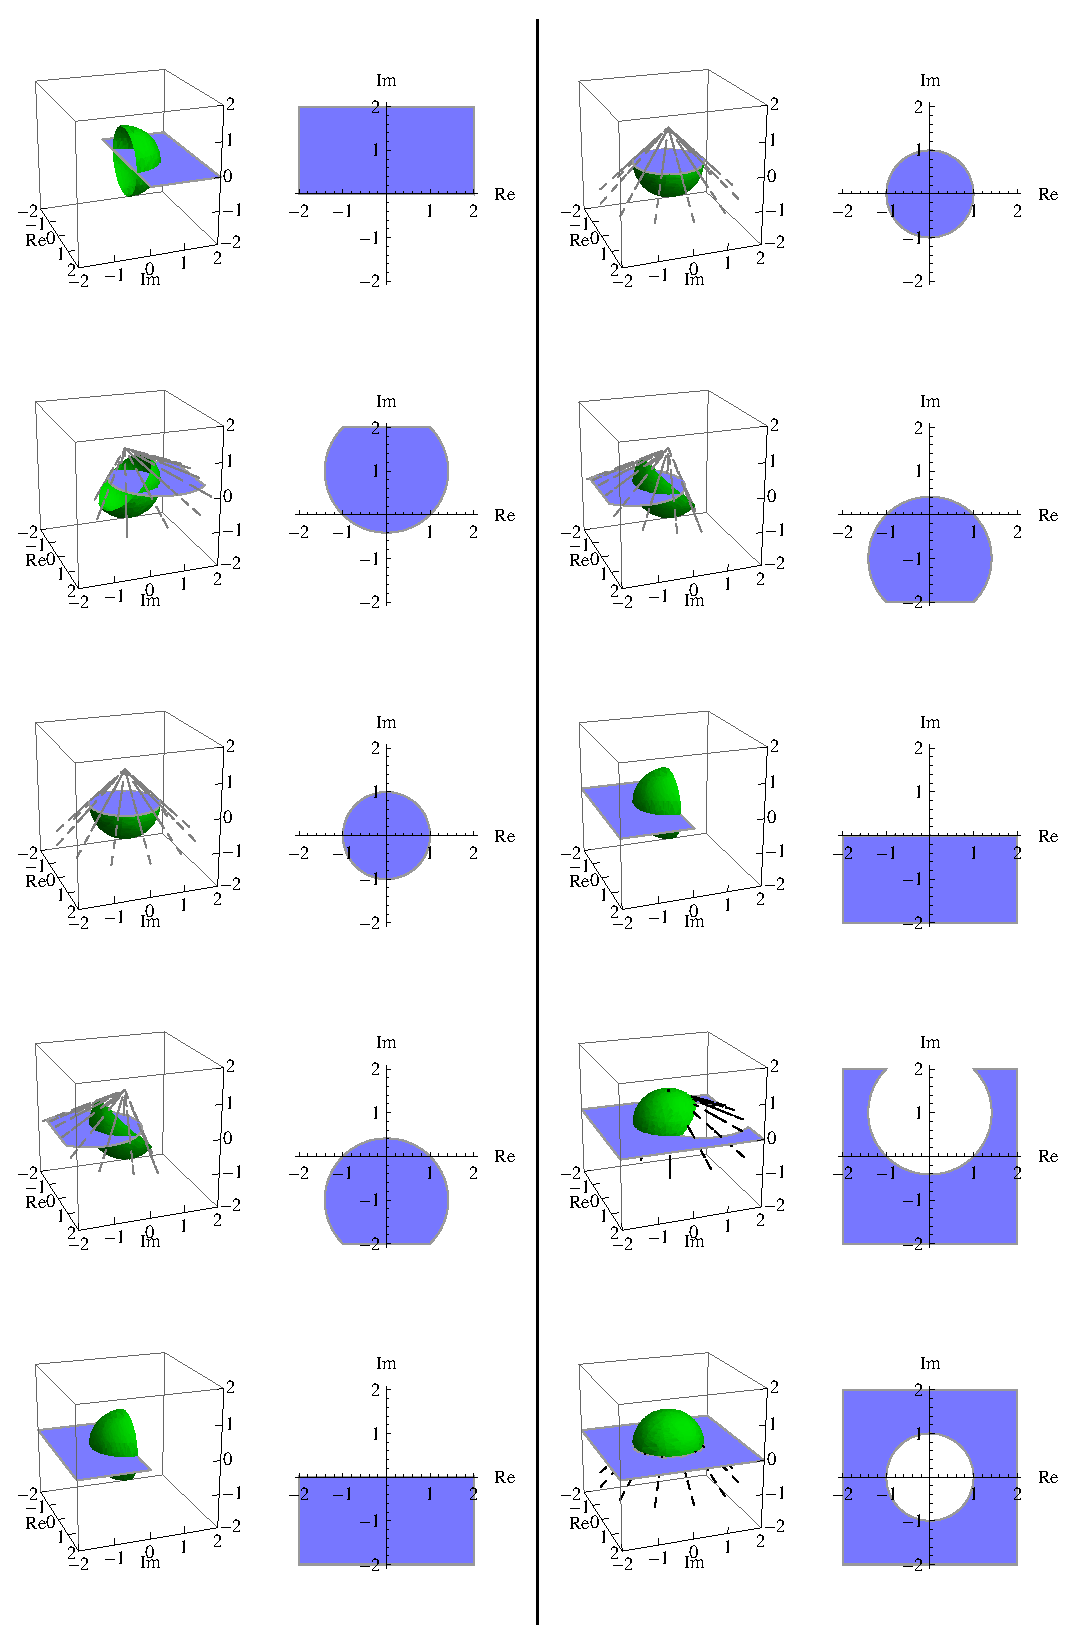
\includegraphics[width=0.9\textwidth]{figures/stereo-proj-1}
\caption[Stereographic projection and the map $z \mapsto \reci{z}$]{Inversion $z \mapsto \reci{z}$ can be interpreted as rotation of the Riemann sphere by $180^{\circ}$ around the $x_1$ axis. It maps the upper to the lower half-plane (left) and the interior of the unit circle to its exterior (right).}
\label{fig_StereoProjInversion}
\end{figure}

\begin{example}
\label{ex_StereoProjInversion}
Consider the map $f: z \mapsto \reci{z}$ and the map $V: \UnitSphere \to \UnitSphere$, which rotates the Riemann sphere around the $x_1$ axis by $180^{\circ}$:
\begin{equation}
\label{eqn_RiemannX1Rotation}
V: x \mapsto
\begin{pmatrix}
1 & \phantom{+}0 & \phantom{+}0 \\
0 & -1           & \phantom{+}0 \\
0 & \phantom{+}0 & -1
\end{pmatrix}
\cdot
\begin{pmatrix}x_1 \\ x_2 \\ x_3 \end{pmatrix}.
\end{equation}
The first row of Figure~\ref{fig_StereoProjInversion} shows the upper half-plane $U$ on the left and the unit disk $D$ on the right together with their images under reverse stereographic projection. We see that both, $U$ and $D$, correspond to a certain ``halfsphere'' of the Riemann sphere. If we rotate these halfspheres around the $x_1$ axis (leaving the points $\{\pm 1\}$ fixed) and continuously perform stereographic projection, we see that after a half turn (in the last row of Figure~\ref{fig_StereoProjInversion}) we end up with the lower half-plane $f(U)$ and the set of points $z$ with $\abs{z} > 1$, $f(D)$. 

It is worth noting that this correspondence between rotation of the Riemann sphere by $180^\circ$ and the map $f : z \mapsto \reci{z}$ does not just hold for the specially chosen sets $U$ and $D$, but indeed pointwise for every $z \in \EC$. In other words, we have
\begin{equation*}
f = P_{\UnitSphere} \circ V \circ P_{\UnitSphere}^{-1}.
\end{equation*}
We show this by a simple calculation, using the fact that $\reci{z} = \frac{\conj{z}}{\abs{z}^2}$ as well as (\ref{eqn_RevStdStereoProj}) and noting that for the case $z = \infty$ limits have to be introduced appropriately:
\begin{IEEEeqnarray*}{rCcCl}
(P_{\UnitSphere}^{-1} \circ f)(z)
&=& \reci{\reci{\abs{z}^2} + 1} 
\begin{pmatrix}
  2 \Re{\reci{z}} \\ 2 \Im{\reci{z}} \\ \reci{\abs{z}^2} - 1
\end{pmatrix}
&=& \frac{\abs{z}^2}{1 + \abs{z}^2}
\begin{pmatrix}
  2 \reci{\abs{z}^2} \Re{\conj{z}} \\
  2 \reci{\abs{z}^2} \Im{\conj{z}} \\
  \frac{1 - \abs{z}^2}{\abs{z}^2}
\end{pmatrix} 
\\
&=&\reci{\abs{z}^2 + 1}
\begin{pmatrix}
  \phantom{+}2 \Re{z} \\ -2 \Im{z} \\ -\abs{z}^2 + 1
\end{pmatrix}
&=&
(V \circ P_{\UnitSphere}^{-1})(z).
\end{IEEEeqnarray*}
\end{example}

\begin{remark}
\label{rem_TRotation}
Other examples for transformations corresponding to a half-turn of the Riemann sphere are $z \mapsto -z$ (rotation around the $x_3$ axis) and $T: z \mapsto -\reci{z}$ (rotation around the $x_2$ axis; as product of half turns around the $x_1$ and $x_3$ axes). $T$ is a function which maps the upper half-plane to itself and which will be important in the study of the modular group in Section~\ref{sec_ModularGroupGenRel}.  
\end{remark}

\begin{figure}
\centering
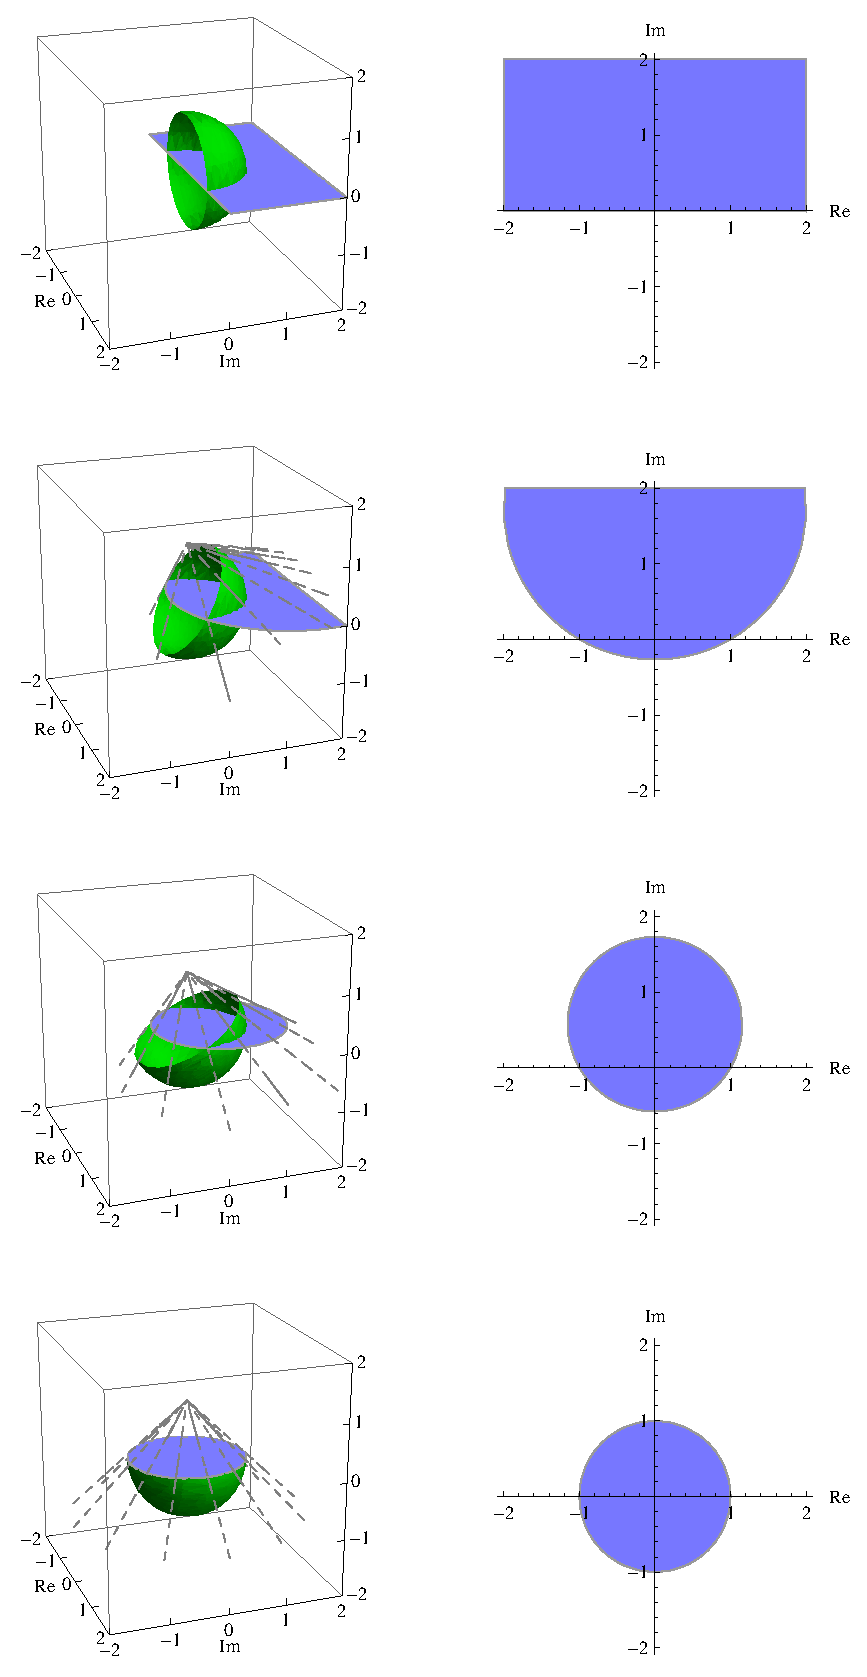
\includegraphics[width=0.7\textwidth]{figures/stereo-proj-2}
\caption[Stereographic projection and the modified Cayley transform]{The modified Cayley transform $z \mapsto \moebius{\ii}{1}{}{\ii}{z}$ maps the upper half-plane to the unit disk, leaving the points $\{\pm 1\}$ fixed. It can be considered as a quarter turn of the Riemann sphere around the $x_1$ axis.}
\label{fig_StereoProjModCayley}
\end{figure}

\begin{example}[Modified Cayley transform]
\label{ex_ModCayleyTransform}
\label{ex_StereoProjCayleyMap}
\index{Modified Cayley transform}
\index{Cayley transform}
In Figure~\ref{fig_StereoProjModCayley}, the action of yet another interesting transformation can be seen, which maps the upper half-plane to the unit disk. It is given by
\begin{equation}
\label{eqn_ModCayleyTransform}
\ModCayley(z) = \moebius{\ii}{1}{}{\ii}{z}
\end{equation}
and can be either considered as a quarter turn of the Riemann sphere around the $x_1$ axis or as ``half of an inversion'', since indeed $\ModCayley^2(z) = \ModCayley(\ModCayley(z)) = \reci{z}$ (compare with left column of Figure~\ref{fig_StereoProjInversion}). In contrast to its better known brother, the \emph{Cayley transform} given by
\begin{equation}
\label{eqn_CayleyTransform}
\Cayley(z) = \frac{z - \ii}{z + \ii} = -\ii \ModCayley(z),
\end{equation}
$\ModCayley$ leaves the points $\{\pm 1\}$ fixed, which often beneficial for visualization purposes. We will call $\ModCayley$ the \emph{modified Cayley transform}. 
\end{example}
\begin{remark} 
Also the Cayley transform $\Cayley$ can be seen as rotation of the Riemann sphere by $120^\circ$ around the axis which is spanned by the vector $(1,-1,1) \in \R^3$. A figure illustrating this fact can be found for example in \Mumford{}, p.\ 88.
\end{remark}

We have now seen exemplary that quite a few interesting maps are induced by rotations of the Riemann sphere. If we are willing to allow not only rotations but also translations of the Riemann sphere, we indeed obtain a new characterization of M�bius transformations, as stated in the next theorem.

\begin{definition}
\index{Rigid motion}
A \emph{rigid motion} of $\R^3$ is an affine transformation of $\R^3$ which is obtained purely by composition of rotations and translations.
\end{definition}

\begin{theorem}[M�bius transformations revealed]
\label{thm_MoebiusRevealed}
A function $\phi : \EC \to \EC$ is a M�bius transformation, if and only if it can be obtained by reverse stereographic projection of $\EC$ to an admissible sphere $S \subseteq \R^3$, followed by a rigid motion T of $\R^3$ which maps $S$ to another admissible sphere $TS$, followed by stereographic projection from $TS$ back to $\EC$:
\begin{equation}
\label{eqn_MoebiusRevealedForm}
\phi = P_{TS} \circ T \circ P_S^{-1}.
\end{equation}
\end{theorem}
\begin{proof}[Sketch of proof]
The fact that all maps of form ($\ref{eqn_MoebiusRevealedForm}$) are indeed M�bius transformations can be seen either by direct calculation or by the observation that $\phi$ corresponds to the map $P_S^{-1} \circ \phi \circ P_S = P_S^{-1} \circ P_{TS} \circ T$ from $S$ to itself. If we identify $S$ with the Riemann sphere, we can regard $\phi$ as a holomorphic automorphism of the Riemann sphere which is therefore a M�bius transformation.

\todo{31}{Literature reference}

It remains to show that every given transformation can indeed be realized in the form (\ref{eqn_MoebiusRevealedForm}). For this purpose, we first consider the four basic types of M�bius transformations:
\begin{description}
\item[Translation:] The map $z \mapsto z + \alpha,\ \alpha \in \C$ can be realized by choosing an arbitrary admissible sphere $S$ and setting $T = T_{\alpha}: x \mapsto x + \iota(\alpha)$, which simply translates $S$ in a direction parallel to the $x_3 = 0$ plane by $\iota(\alpha)$.
\item[Dilation:] The map $z \mapsto \rho z,\ \rho > 0$ can be obtained by choosing an arbitrary admissible sphere with north pole $n$ and setting $T = D_{\rho}: x \mapsto x + \left(0, 0, (\rho-1) n_3\right)$, which moves $S$ up- ($\rho > 1$)  or downwards ($\rho < 1$) in $x_3$ direction.
\item[Rotation:] The map $z \mapsto \epo{\ii \theta} z,\ \theta \in (-\pi, \pi]$ can be realized by choosing an arbitrary admissible sphere and setting 
\begin{equation*}
T = R_{\theta}: x \mapsto 
\begin{pmatrix}
\cos{\theta} & -\sin{\theta}            & 0\\
\sin{\theta} & \phantom{+}\cos{\theta}  & 0\\
0            & \phantom{+}0             & 1
\end{pmatrix}
\cdot
\begin{pmatrix}x_1 \\ x_2 \\ x_3 \end{pmatrix},
\end{equation*}
which rotates $S$ around the $x_3$ axis by an angle of $\theta$.
\item[Inversion:] We have seen in Example~\ref{ex_StereoProjInversion} that the map $z \mapsto \reci{z}$ can be realized by choosing $S$ as the unit sphere $\UnitSphere$ and setting $T = V$ -- as defined in (\ref{eqn_RiemannX1Rotation}) -- which is a rotation of $\UnitSphere$ around the $x_1$ axis by an angle of $180^{\circ}$.
\end{description}
Now let $\phi(z) = \moebius{a}{b}{c}{d}{z}$ be an arbitrary M�bius transformation. As in the proof of Lemma~\ref{lem_MoebiusGenerators}, if $c = 0$ we may assume without restriction that $d = 1$ and therefore $\phi(z) = az + b$. Clearly this map can be realized in the form (\ref{eqn_MoebiusRevealedForm}) by starting with an arbitrary admissible sphere $S$ and taking $T$ as the composition of rotation by $\arg(a)$, dilation by $\abs{a}$ (in either order), followed by translation by $b$:
\begin{equation*}
T := T_b \circ D_{\abs{a}} \circ R_{\arg(a)}.
\end{equation*}
If $c \ne 0$, we can scale the coefficients $a,b,c,d$ such that $c = 1$ and write $\phi$ in the form
\begin{equation*}
\phi(z) = a + \frac{b - ad}{z + d}.
\end{equation*}
Now we choose $S$ to be the sphere with unit radius centered at the point $\iota(-d)$ and we compose $T$ out of the following rigid motions: First, translation by $d$ transforms $S$ to the unit sphere $\UnitSphere$. Thus we can indeed apply $V$ as the second transformation in order to perform an inversion. Finally we apply rotation and dilation by the factor $b - ad$ followed by a translation by $a$:
\begin{equation*}
T := T_a \circ D_{\abs{b - ad}} \circ R_{\arg(b - ad)} \circ V \circ T_d. \qedhere
\end{equation*}
\end{proof}


% --------------------------------------------- Subsection: Generalized circles
\subsection{Generalized circles}

\index{Generalized!circle}
From the geometric point of view, M�bius transformations have the beautiful property that they preserve generalized circles. \emph{Generalized circles} are either circles (in the usual sense) or lines on the complex plane $\C$. They can also be thought of circles on the Riemann sphere (\ie the extended complex plane $\EC$ projected to the unit sphere $\UnitSphere$, see Remark~\ref{rem_RiemannSphere}), where lines on the complex plane stand in a one-to-one correspondence to circles through the point $\infty$ on the Riemann sphere. In order to give an exact definition, we first make the following considerations:

A circle with center $m \in \C$ and radius $r > 0$ can be described as the set of points $z \in \C$ for which
\begin{equation*}
\abs{z - m} = r.
\end{equation*}
This is obviously equivalent to
\begin{equation*}
\abs{z - m}^2 = (z - m) \conj{(z - m)} = r^2
\end{equation*}
and
\begin{equation}
\label{eqn_Circle}
z \conj{z} - m \conj{z} - \conj{m} z + m \conj{m} - r^2 = 0.
\end{equation}
The generalization comes into play if we multiply this last equation by a constant $A \in \R$
\begin{equation*}
A z \conj{z} - A m \conj{z} - A \conj{m} z + A m \conj{m} - A r^2 = 0
\end{equation*}
and introduce constants $B$, $C$ and $D$ appropriately such that we can write it in the form
\begin{equation}
\label{eqn_GenCircle}
A z \conj{z} + B \conj{z} + C z + D = 0.
\end{equation}
Note that $D$ is real and $B = \conj{C}$ are complex conjugates. From an equation of form (\ref{eqn_GenCircle}) we can read off the center and radius of the corresponding circle by
\begin{IEEEeqnarray}{rCl}
m &=& -\frac{B}{A}, \IEEEyessubnumber \\
r &=& \sqrt{m \conj{m} - \frac{D}{A}} = \sqrt{\frac{BC - AD}{A^2}}. \IEEEyessubnumber
\end{IEEEeqnarray}
Clearly we can only do so, if $A \ne 0$ and $BC - AD > 0$. 

In the case when $A = 0$, equation (\ref{eqn_GenCircle}) can be written as
\begin{equation*}
\Re{\frac{C}{\abs{C}} z} = -\frac{D}{2 \abs{C}},
\end{equation*}
which defines a line on the complex plane. We see this by considering the simpler equation $\Re{z} = -\frac{D}{2 \abs{C}}$ first (we omit the factor $\frac{C}{\abs{C}}$), which obviously defines a line parallel to the imaginary axis through the real point $-\frac{D}{2 \abs{C}}$. Then we observe that the multiplication with $\frac{C}{\abs{C}}$ just rotates this line clockwise around the origin by an angle which is given by $\arg(C)$.

To conclude our considerations, we note that equation (\ref{eqn_GenCircle}) can also be written in matrix form:
\begin{equation*}
\rvec{\conj{z}}{1} \cdot \mat{A}{B}{C}{D} \cdot \cvec{z}{1} = 0.
\end{equation*}
The matrix in this equation has a negative determinant, because of the condition $BC - AD > 0$ from above. Moreover, it is a Hermitian matrix, a notion which we will shortly recall:
\begin{definition}
\label{dfn_HermitianMatrix}
\index{Hermitian!matrix}
\index{Hermitian!transpose}
\index{Conjugate transpose}
Let $n > 0$ and $M \in \Mat{\C}{n}{n}$. The matrix
\begin{equation*}
\htransp{M} := \transp{\overline{M}}
\end{equation*}
obtained by complex conjugation and transposition of $M$ is called \emph{Hermitian transpose} or \emph{conjugate transpose} of $M$. If $M$ has the property $\htransp{M} = M$, it is called a \emph{Hermitian} matrix.
\end{definition}
Having now the right vocabulary at hand, we can give an exact definition for generalized circles.
\begin{definition}
Let $M = \smallmat{A}{B}{C}{D} \in \Mat{\C}{2}{2}$ be a Hermitian matrix with $\det(M) < 0$. A \emph{generalized circle} is the set of solutions $z \in \C$ to
\begin{equation}
\label{eqn_GenCircleMat}
\rvec{\conj{z}}{1} \cdot M \cdot \cvec{z}{1} = 0
\end{equation}
plus eventually the point $\infty$, if and only if $A = 0$, \ie when the generalized circle corresponds to a line on the complex plane.
\end{definition}

\begin{remark}
Since there should be no danger of confusion, we will from now on use the same name for a generalized circle and its corresponding Hermitian matrix (which is uniquely determined up to a real scalar factor).
\end{remark}

\begin{remark}
\label{rem_GeneralizedDisk}
\index{Generalized!disk}
One could easily do the same thing as above starting with the equations
\begin{equation*}
\abs{z - m} < r \quad \text{or} \quad  
\abs{z - m} \le r
\end{equation*}
instead of $\abs{z - m} = r$, which naturally leads to the notions of open or closed \emph{generalized disks}, determined by
\begin{equation}
\rvec{\conj{z}}{1} \cdot M \cdot \cvec{z}{1} < 0 \quad \text{or} \quad
\rvec{\conj{z}}{1} \cdot M \cdot \cvec{z}{1} \le 0.
\end{equation}
\end{remark}

\begin{theorem}
\label{thm_MoebiusGenCircle}
Let $M \in \Mat{\C}{2}{2}$ be a Hermitian matrix with $\det(M) < 0$ and $P \in \GL{\C}$. The image of the generalized circle $M$ under the M�bius transformation $\phi$ corresponding to the matrix $P \in \GL{\C}$ is the generalized circle  $\htransp{(\inv{P})} \cdot M \cdot \inv{P}$.
\end{theorem}
\begin{proof}
Let us write $P = \smallmat{a}{b}{c}{d}$, such that the corresponding M�bius transformation $\phi$ has the form
\begin{equation*}
\phi(z) = \moebius{a}{b}{c}{d}{z}.
\end{equation*}
Now we set $w = \phi(z)$ and show that 
\begin{equation*}
\rvec{\conj{z}}{1} \cdot M \cdot \cvec{z}{1} = 0
\end{equation*}
if and only if
\begin{equation*}
\rvec{\conj{w}}{1} \cdot \htransp{(\inv{P})} \cdot M \cdot \inv{P} \cdot \cvec{w}{1} = 0.
\end{equation*}
But this follows immediately from
\begin{equation*}
P \cdot \cvec{z}{1} = \cvec{a z + b}{c z + d} = (c z + d) \cvec{w}{1}.\qedhere
\end{equation*}
\end{proof}




% ------------------------------------------------------ CHAPTER: MODULAR GROUP
\chapter{The modular group}

% ---------------------------------------------- Section: Generators, Relations
\section{The modular group}

Throughout this section and also later, we adopt the notation of Schoeneberg \cite{schoeneberg1974elliptic}.

\begin{definition}
\label{dfn_ModularGroup}
\index{Modular!group}
\index{Modular!transformation}
\index{Inhomogeneous!modular transformation}
A M�bius transformation $\phi$ of the form
\begin{equation*}
\phi(z) = \moebius{a}{b}{c}{d}{z},\quad a,b,c,d \in \Z,\quad ad - bc = 1
\end{equation*}
is called \emph{(inhomogeneous) modular transformation}.
\end{definition}

\begin{theorem}
\label{thm_ModularGroup}
\index{Modular!group}
The set of modular transformations forms a discrete subgroup of the group of M�bius transformations and can be identified with the projective special linear group $\PSL{\Z}$. This group is called the \emph{modular group} and is denoted by $\ModGrp$.
\end{theorem}
\begin{proof}
The proof is very similar to that of Theorem \ref{thm_MoebiusGroup}. The only thing which has to be changed is the homomorphism $\pi$ defined in (\ref{eqn_homPi}). Its domain now is $\SL{\Z}$, the group of 2-by-2 matrices over $\Z$ with determinant 1, rather than $\GL{\C}$ (or $\SL{\C}$). Again it follows by the first isomorphism theorem, that the modular group $\ModGrp$ is isomorphic to $\SL{\Z} / \ker(\pi) \cong \PSL{\Z}$. The fact that $\ModGrp$ is a discrete subgroup of the group of M�bius transformations is now also directly evident.
\end{proof}

\begin{remark}
\index{Inhomogeneous!modular transformation}
\index{Homogeneous!modular transformation}
\index{Modular!transformation}
The elements of $\SL{\Z}$ are often called \emph{homogeneous modular transformations}, whereas the transformations of $\ModGrp = \PSL{\Z}$ are called \emph{inhomogeneous}. Strictly seen, an inhomogeneous transformation has to be denoted as $[M]_{\sim}$, which is the equivalence class in $\PSL{\Z}$ of a matrix $M \in \SL{\Z}$. It is clear, that $[M]_{\sim}$ is nothing but the set $\{\pm M\}$ and again for easier notation, we will from now on simply write either $M$ or $-M$ instead of $[M]_{\sim}$.
\end{remark}

\todo{16}{Basic mapping properties}

\subsection{Generators and relations}

In group theory it is an important question, which systems of group elements and relations (in the sense of definition \ref{dfn_GrpConstructGenRel}) completely describe the structure of any given group. This section is devoted to the answer of this question in the case of the modular group.

Before we start, we introduce the following modular transformations which will serve as group generators:

\begin{IEEEeqnarray*}{RL}
U: & z \mapsto z + 1 \\
T: & z \mapsto -\reci{z} \\
R = TU: & z \mapsto -\reci{z + 1}
\end{IEEEeqnarray*}

\begin{remark}
Sadly, in literature there is no consensus about the notation of these transformations. We use the notation of Schoeneberg \cite{schoeneberg1974elliptic} here, but other notations are frequent. In Klein/Fricke \cite{klein1966vorlesungen}, the symbol $S$ is used instead of $U$ and in other literature as well as on Wikipedia, additionally the roles of $S$ and $T$ are swapped.
\end{remark}

\begin{theorem}
\label{thm_ModGrpGen}
The modular group is generated by the elements $U: z \mapsto z+1$ and $T: z \mapsto -\reci{z}$. 
\end{theorem}
\begin{proof}
Let $A: z \mapsto \moebius{a}{b}{c}{d}{z}$ be an arbitrary modular transformation. Our goal is to show that $A$ can be written as product of the transformations $U$ and $T$. For this purpose it is more convenient to view these transformations as elements of $\PSL{\Z}$, namely
\begin{equation*}
A = \mat{a}{b}{c}{d}, \quad U = \mat{1}{1}{0}{1}, \quad T = \mat{0}{-1}{1}{\phantom{+}0}.
\end{equation*}

Let's first consider the two special cases, when $a$ or $c$ are zero. If $a=0$, it follows from $ad - bc = 1$, that $-b = c = \pm 1$.  Therefore we have
\begin{equation*}
A \sim c A = \mat{0}{-1}{1}{c d} = TU^{c d}.
\end{equation*}
Similarly, $c = 0$ gives $a = d = \pm 1$ and
\begin{equation*}
A \sim a A = \mat{1}{a b}{0}{1} = U^{a b}.
\end{equation*}
In the general case, when $a$ and $c$ are both nonzero, $ad - bc = 1$ implies that $a$ and $c$ are coprime and the Euclidean algorithm therefore yields
\begin{eqnarray*}
      a &=& q_0 \cdot c\phantom{_0} + r_1 \\
      c &=& q_1 \cdot r_1 + r_2 \\
    r_1 &=& q_2 \cdot r_2 + r_3 \\
        &\vdots& \\
r_{n-1} &=& q_n \cdot r_n + r_{n+1}\\
        &=& q_n \cdot 1\phantom{_n} + 0.
\end{eqnarray*}
We can use this to reduce the Matrix $A$ by successively multiplying powers of $U$ and $T$ from the left. Just note, that multiplication with $U^k$ adds $k$ times the second row to the first row, whereas $T$ swaps the rows and changes the sign of one arbitrary row\footnote{This freedom of choice is again due to the fact that the matrices $M$ and $-M$ represent the same element in $\PSL{\Z}$.}. If we concentrate only on the first column of $A$ and apply the first few transformations
\begin{equation*}
\cvec{a}{c}                           \overset{U^{-q_0}}{\longmapsto}
\cvec{r_1}{c\phantom{_1}}             \overset{T}{\mapsto} 
\cvec{\phantom{+}c\phantom{_1}}{-r_1} \overset{U^{q_1}}{\longmapsto}
\cvec{\phantom{+}r_2}{-r_1}           \overset{T}{\mapsto} 
\cvec{r_1}{r_2}                       \overset{U^{-q_2}}{\longmapsto}
\cvec{r_3}{r_2}                       \overset{T}{\mapsto}
\cvec{\phantom{+}r_2}{-r_3}           \mapsto \dots,
\end{equation*}
we soon recognize the general mapping rule, which is
\begin{IEEEeqnarray*}{rCll}
\cvec{\phantom{+}r_{j-1}}{\phantom{+}r_{j\phantom{+0}}} 
& \overset{TU^{-q_j}}{\longmapsto}
& \cvec{\phantom{+}r_{j\phantom{+0}}}{-r_{j+1}}
& \quad \text{for even } j \text{ and}\\
\cvec{\phantom{+}r_{j-1}}{-r_{j\phantom{+0}}}
& \overset{TU^{q_j}}{\longmapsto}
& \cvec{\phantom{+}r_{j\phantom{+0}}}{\phantom{+}r_{j+1}} 
& \quad \text{for odd } j.
\end{IEEEeqnarray*}
When we set $r_{-1} := a$ and $r_0 := c$, this rule is true for $0 \le j \le n$. Obviously the described procedure ends with
\begin{equation*}
\cdots \overset{T}{\mapsto}
\cvec{\phantom{+}r_{n\phantom{+0}}}{\pm r_{n+1}} = \cvec{1}{0}.
\end{equation*} 
Because we know the first column of the resulting matrix and its determinant, which is 1, we can conclude that for some $k \in \Z$ it must have the form
\begin{equation*}
\mat{1}{k}{0}{1} = U^k.
\end{equation*}
By setting $e_n := (-1)^{n} q_n$, we therefore have 
\begin{equation*}
TU^{-e_n} TU^{-e_{n-1}} \cdots TU^{-e_1}TU^{-e_0} A = U^k
\end{equation*}
or equivalently,
\begin{equation*}
A = U^{e_0} TU^{e_1} \cdots TU^{e_{n-1}} TU^{e_n} T U^k,
\end{equation*}
which gives the desired representation of $A$ in terms of $U$ and $T$ in the case when $a$ and $c$ are both non-zero.
\end{proof}

It is worth formulating the algorithm used in the previous proof explicitly in the following corollary.
\begin{corollary}
\label{cor_ModGrpTUAlg}
An arbitrary modular transformation $A: z \mapsto \moebius{a}{b}{c}{d}{z}$ can be represented in terms of the transformations $U: z \mapsto z+1$ and $T : z \mapsto -\reci{z}$, by performing the following steps:
\begin{enumerate}
\item If $a = 0$, then $A = TU^{c d}$ and if $c = 0$, then $A = U^{a b}$ and we are done. Otherwise, continue with \ref{itm_ModGrpTUAlgStart}.
\item \label{itm_ModGrpTUAlgStart} Apply the Euclidean algorithm to $a$ and $c$ with the first division being $a = q_0 \cdot c + r_1$ ($q_0$ may be $\le 0$) and let $n$ be the number of the  last division (start counting from 0). Call the arising quotients $q_0,q_1,\dots,q_n$.
\item For $j \in \{0,1,\dots,n\}$ set $e_j := (-1)^j q_j$.
\item Calculate the matrix product $TU^{-e_n} TU^{-e_{n-1}} \cdots TU^{-e_1}TU^{-e_0} A$ and multiply by $\pm 1$ in order to obtain a representation with positive diagonal elements. Read off the right-upper entry and call it $k$.
\end{enumerate}
The transformation $A$ can now be written as
\begin{equation}
\label{eqn_ModGrpTUAlg}
A = U^{e_0} TU^{e_1} \cdots TU^{e_{n-1}} TU^{e_n} T U^k.
\end{equation}
\end{corollary}

We have seen that $U$ and $T$ generate the modular group, but it is not yet clear, which group words in $U$ and $T$ give the same modular transformations. For example, it is easy to see that $T^2 = 1$ and $(TU)^3 = 1$ are relations satisfied by $T$ and $U$. Before we can show, that these two relations are ``the only ones'', \ie all other relations can be derived from them, we need the following Lemma:

\begin{lemma}
Let $a, b, c, d \in \Z$ be arbitrary integers satisfying $ad - bc = 1$. Then one, and only one of the following three conditions is true:
\begin{IEEEeqnarray*}{RRCCCRCC}
  (i)\quad & ac       &\ge& 0 &\quad\land\quad&       bd &\ge& 0\\
 (ii)\quad & a^2 + ac &\le& 0 &\quad\land\quad& b^2 + bd &\le& 0\\
(iii)\quad & c^2 + ac &\le& 0 &\quad\land\quad& d^2 + bd &\le& 0
\end{IEEEeqnarray*}
\end{lemma}
\begin{proof}
It is trivial to see, that $(i)$ implies $\lnot (ii)$ and $\lnot (iii)$. It therefore remains to show, that $\lnot(i)$ implies either $(ii)$ or $(iii)$.
\end{proof}

\begin{theorem}
\label{thm_ModGrpRel}
The generators $T: z \mapsto -\reci{z}$ and $R: z \mapsto -\reci{z+1}$ of the modular group satisfy the relations
\begin{equation}
\label{eqn_ModGrpTRRel}
T^2 = \id{\C}, \quad R^3 = \id{\C}
\end{equation}
and all other relations are derived from these two. Therefore the modular group is isomorphic to the free product of a cyclic group of order 2 and a cyclic group of order 3.
\end{theorem}

\todo{18}{Proof}

% ------------------------------- Subsection: Fundamental domains, tessellation
\subsection{The fundamental domain and the tessellation of the halfplane}

\begin{figure}
\centering
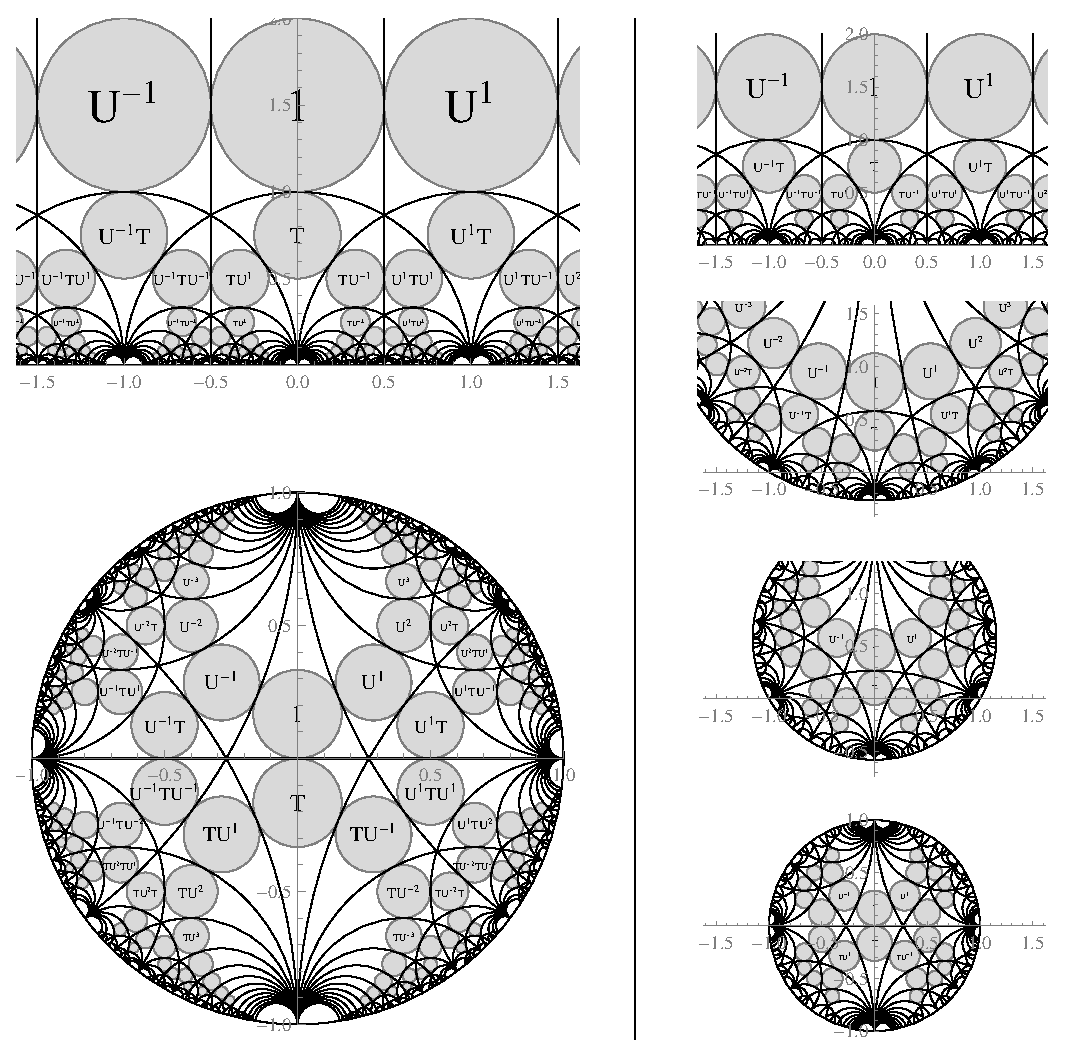
\includegraphics[width=\textwidth]{figures/modular-tiling-1}
\caption{The tessellation of the upper halfplane.}
\label{fig_ModularTiling}
\end{figure}


\todo{25}{Definition, description and figures}


% --------------------------------------------- Subsection: Hyperbolic geometry
\subsection{Hyperbolic geometry}

\todo{11}{Connection to hyperbolic geometry (disk/halplane model)}


% ------------------------------- Subsection: Ford circles, continued fractions
\subsection{Ford circles and continued fractions}

For an arbitrary modular transformation $A$, a representation as product of shifts $U^j: z \mapsto z+j$ and inversions $T: z \mapsto -\reci{z}$ can be found by the algorithm described in Corollary \ref{cor_ModGrpTUAlg}. By writing out this product, for example in the case when $n=2$, we have
\begin{equation*}
A = U^{e_0}T U^{e_1}T U^{e_2}T U^k,
\end{equation*}
or more explicitly
\begin{equation}
\label{eqn_ALongConFrac}
A(z) = e_0 - \reci{e_1 - \reci{e_2 - \reci{k + z}}}.
\end{equation}
\index{Continued fraction}
Here, a close relation between modular transformations and continued fractions immediately gets apparent. In this section we will investigate this relation somewhat deeper. 
First, we will use Pringsheim's more space-saving notation for continued fractions, namely
\begin{equation}
\label{eqn_ConFracNotation}
b_0 + \frac{a_1}{b_1 + \frac{a_2}{b_2 + \frac{a_3}{b_3 + \dots}}} =: 
b_0 + \cfr{a_1}{b_1} + \cfr{a_2}{b_2} + \cfr{a_2}{b_3} + \dots
\end{equation}
In the case when all $a_j = 1$, we adhere to the standard sequence notation for continued fractions:
\begin{equation*}
b_0 + \reci{b_1 + \reci{b_2 + \dots}} =: [b_0,b_1,b_2,\dots].
\end{equation*}
We can now reformulate Corollary \ref{cor_ModGrpTUAlg} in order to construct a continued fraction representation of any given modular transformation.

\begin{corollary}
An arbitrary modular transformation $A(z) = \moebius{a}{b}{c}{d}{z}$ can be written as continued fraction
\begin{equation}
\label{eqn_ModTransConFrac}
A(z) = [q_0,q_1,\dots,q_n,(-1)^{n+1}(k+z)]
\end{equation}
where the integers $n$, $q_0,q_1,\dots,q_n$ and $k$ are determined by the algorithm described in Corollary \ref{cor_ModGrpTUAlg}.
\end{corollary}
\begin{proof}
By using the continued fraction representation of $A$ given in (\ref{eqn_ALongConFrac}) and by applying the definition $e_j$ := $(-1)^j q_j$ we see
\begin{IEEEeqnarray}{rCcCcCcCcCcCc}
A(z) &=& e_0 &+& \cfr{-1}{e_1} 
          &+& \cfr{-1}{e_2} 
          &+& \dots 
          &+& \cfr{-1}{e_n} 
          &+& \cfr{-1}{k + z} \nonumber \\
  &=& q_0 &+& \cfr{-1}{-q_1} 
          &+& \cfr{-1}{q_2} 
          &+& \dots 
          &+& \cfr{-1}{(-1)^n q_n} 
          &+& \cfr{-1}{k + z}. \label{eqn_ModTransConFracInterim}
\end{IEEEeqnarray}
Now for every odd $j \le n$ we can rewrite 
\begin{equation*}
\cfr{-1}{-q_j} + \cfr{-1}{\dots} \quad \text{to} \quad \cfr{1}{q_j} + \cfr{1}{\dots}.
\end{equation*}
Thus if $n$ is odd, every numerator $-1$ in (\ref{eqn_ModTransConFracInterim}) can be turned into $+1$. In the other case, when $n$ is even, only one negative numerator at the end, $\frac{-1}{k+z}$, remains, but this can easily be rewritten to $\frac{1}{-(k+z)}$. Taking both cases together, we obtain (\ref{eqn_ModTransConFrac}).
\end{proof}

\begin{figure}
\centering
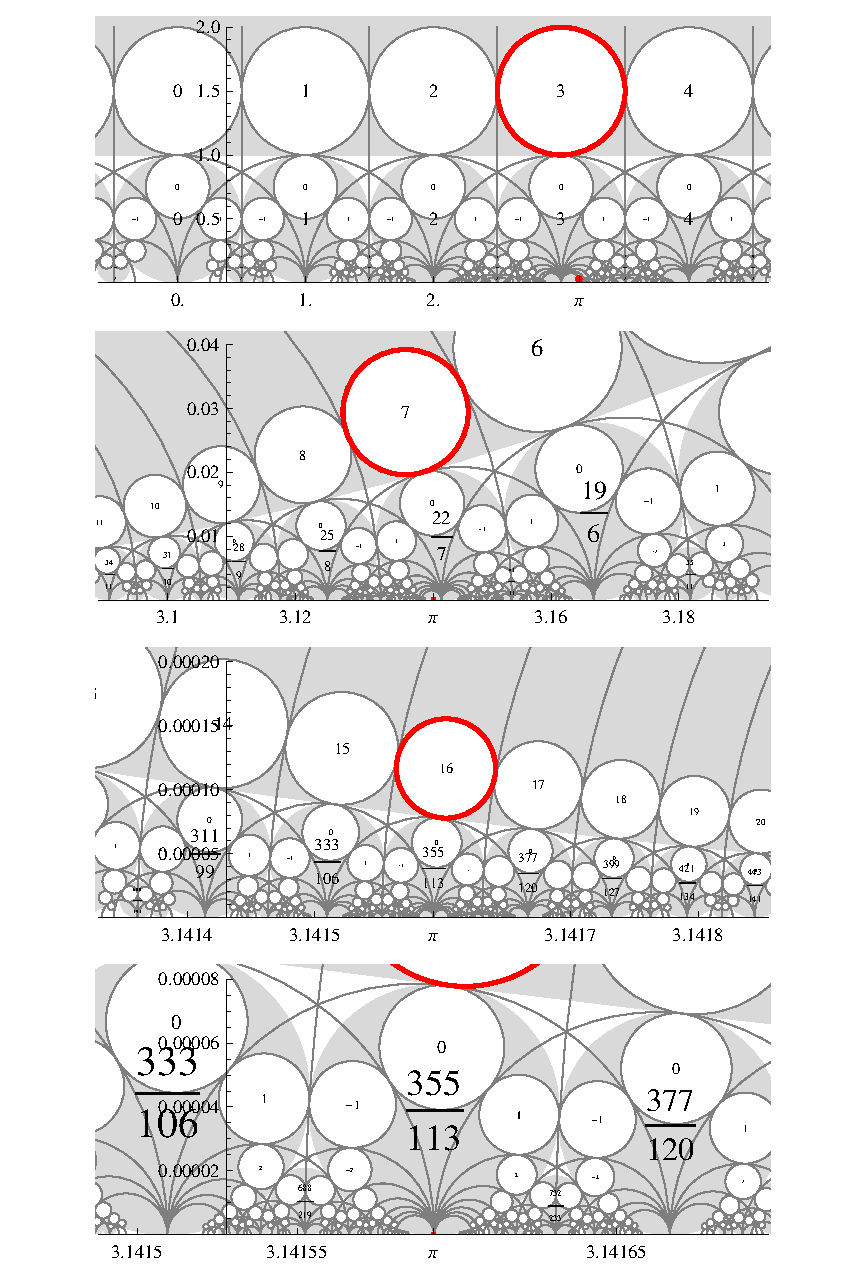
\includegraphics[width=\textwidth]{figures/cont-frac-pi}
\caption{$\pi = \frac{355}{113}$ -- well, almost.}
\label{fig_ContFracPi}
\end{figure}


\todo{19}{The modular group and ford circles}




% ------------------------------------------------ Section: Fundamental Domains 
\section{Fundamental sets and regions}

We have seen in Remark~\ref{rem_NatureMoebius} that considering M�bius transformations as meromorphic functions $\EC \to \EC$ very naturally induces a group action of $\PGL{\C}$ on $\EC$. Clearly this group action is also given for any subgroup of $\PGL{\C}$ and in particular for the modular group: For $A = \smallmat{a}{b}{c}{d} \in \PSL{\Z}$ the group action is given by
\begin{equation}
\label{eqn_ModGrpAction}
Az := \moebius{a}{b}{c}{d}{z}.
\end{equation}

As usual we call two points $z, w \in \EC$ \emph{equivalent}, in symbols $z \sim w$, if there is a transformation $A \in \PSL{\Z}$ such that $Az = w$. We are now interested in subsets of $\EC$ containing exactly one point from each equivalence class of the relation $\sim$:

\begin{definition}[Fundamental set]
\label{dfn_FundamentalSet}
\index{Fundamental!set}
Let $G$ be a group acting on the set $\mathcal{S}$. Denote equivalence of points in $\mathcal{S}$ under $G$ by $\sim$, as in (\ref{eqn_GroupActionEquivalence}). A subset $\FunSet \subseteq \mathcal{S}$ is called a \emph{fundamental set} with respect to the group action of $G$ on $\mathcal{S}$, if $\FunSet$ contains exactly one point from each orbit $Gx = [x]_\sim$, \ie the map $\FunSet \to \mathcal{S}/\sim$, $x \mapsto [x]_\sim$ is bijective.
\end{definition}

\begin{remark}
Fundamental sets always exist, but they are not unique in any way. If $\FunSet$ is a fundamental set, then for every subset $X \subseteq \FunSet$ and for every $g \in G$, also the set $(\FunSet \setminus X) \cup gX$ is fundamental.
\end{remark}

\begin{remark}
\label{rem_FunSetUniqueElement}
If $\FunSet$ is a fundamental set for the group action of $G$ on $\mathcal{S}$, then by definition for every $x \in \mathcal{S}$ there is a $g \in G$ such that $gx \in \FunSet$. Clearly this element $g$ is unique if and only if the stabilizer $\Stabilizer{G}{gx} = \setdef{h \in G}{hgx = gx}$ is trivial ($\Stabilizer{G}{gx}$ contains just the identity element). Since the groups $\Stabilizer{G}{gx}$ and $\Stabilizer{G}{x} = \setdef{h \in G}{hx = x}$ are conjugate, \ie
\begin{equation*}
\Stabilizer{G}{x} = \inv{g} \cdot \Stabilizer{G}{gx} \cdot g,
\end{equation*}
we conclude that the element $g \in G$ with $gx \in \FunSet$ is unique if and only if the stabilizer $\Stabilizer{G}{x}$ is trivial. Clearly $gx \in \FunSet$ is equivalent to $x \in \inv{g}\FunSet$, which allows us to reformulate the above fact the following way: The images of the fundamental set $\FunSet$ under the group action of $G$ cover the whole set $\mathcal{S}$, that is
\begin{equation*}
\mathcal{S} = \bigcup_{g \in G} g\FunSet.
\end{equation*}
A point $x \in \mathcal{S}$ is covered once, \ie there is a unique $g \in G$ with $x \in g\FunSet$, if and only if $\Stabilizer{G}{x}$ is trivial.
\end{remark}

If -- like in the case of $\EC$ -- the set $\mathcal{S}$ comes together with a topology defined on it, it is often advantageous to use a concept slightly different to fundamental sets:

\begin{definition}[Fundamental region]
\label{dfn_FunDom}
\index{Fundamental!region}
Let $G$ be a group acting on a set $\mathcal{S}$ which is (a subset of) a topological space. A nonempty open subset $\FunDom \subseteq \mathcal{S}$ is called \emph{fundamental region} with respect to the group action of $G$ on $\mathcal{S}$, if it contains no distinct points equivalent under $G$ and if the neighborhood of every boundary point of $\FunDom$ contains a point of $\mathcal{S} \setminus \FunDom$ which is equivalent to a point within $\FunDom$.
\end{definition}

\begin{remark}
The relation between fundamental sets and fundamental regions is the following: If $\FunDom \subseteq \mathcal{S}$ is a fundamental region and if the images under $G$ of its topological closure $\topcl{\FunDom}$ cover the whole set $\mathcal{S}$, \ie 
\begin{equation*}
\mathcal{S} = \bigcup_{g \in G} \topcl{\FunDom},
\end{equation*}
then a fundamental set $\FunSet$ can always be obtained from $\FunDom$ by adjoining certain boundary points of $\FunDom$ and we have $\FunDom \subseteq \FunSet \subseteq \topcl{\FunDom}$.

\index{Discontinuity}
However, a fundamental region must not always exist: Consider the group of translations $z \mapsto z + \alpha$, $\alpha \in \R$, acting on the complex plane $\C$. No matter how we arrange a fundamental set $\FunSet$, take for example the imaginary axis $\Re{z} = 0$, the interior of $\FunSet$ will always be empty and thus cannot be a fundamental region. In fact, a necessary and sufficient condition for the existence of a fundamental region is that the group action is \emph{discontinuous} on $\mathcal{S}$, \ie there exists and \emph{ordinary} point $x \in \mathcal{S}$, meaning that there is no sequence of the form $(g_n y)_{n \ge 0}$ with distinct $g_n \in G$ and arbitrary $y \in \mathcal{S}$ which converges to $x$ -- see \Lehner{}, Chapter IV, 1B.

Note that in \Schoeneberg{}, the term ``fundamental region'' is used for any set $X$ containing a fundamental set $\FunSet$ plus some or all of its (remaining) boundary points. We prefer the above definition for being more close to the commonly used meaning of ``region'', \ie a topologically connected and open set. However, we emphasize that according to our definition a fundamental region does not need to be topologically connected. 
\end{remark}

The goal of the remainder of this section is to identify fundamental regions and fundamental sets for the action of the modular group on $\EC$. For this purpose it is instructive to first consider homogeneous modular transformations and their natural action on $\C^2$.

% -------------------------------------------- Subsection: The action of SL2(Z)
\subsection{The action of $\SL{\Z}$ on $\C^2$}

The homogeneous modular group $\SL{\Z}$ naturally acts on the vector space $\C^2$ by matrix-vector multiplication. Written out explicitly, for $A \in \SL{\Z}$ and $x = ({}^u_v) \in \C^2$, this group action is given by
\begin{equation*}
A x = \mat{a}{b}{c}{d} \cvec{u}{v} = \cvec{a u + b v}{c u + d v}.
\end{equation*}
We equip $\C^2$ with the standard Euclidean norm: 
\begin{equation*}
\eucnorm{x} := \sqrt{\abs{u}^2 + \abs{v}^2}.
\end{equation*}
Let us denote the orbit of $x$ under $\PSL{\Z}$ by 
\begin{equation}
O_x := \PSL{\Z} x = \setdef{Ax}{A \in \SL{\Z}} \subseteq \C^2.
\end{equation}
We now wish to find a fundamental set (or at least a fundamental region) with respect to action of $\SL{\Z}$ on $\C^2$. For this purpose, we need to choose exactly one vector $\tilde{x}$ from each of the orbits $O_x$, $x \in \C^2$. In order to restrict the number of candidate vectors to an easily manageable number, we could try to first look just at vectors with minimal $\eucnorm{\cdot}$-norm in $O_x$. The problem with this is that in general the orbit $O_x$ might contain vectors of arbitrary small $\eucnorm{\cdot}$-norm -- in other words $\min{\eucnorm{O_x}}$ might in general not necessarily exist. However, in many cases it does:

\begin{lemma}
\label{lem_SL2FunDomMinExists}
Let $x = ({}^u_v) \in \C^2$ be a vector with $u \conj{v} \notin \R$. For every $r > 0$, there are only finitely many points $y \in O_x$ with $\eucnorm{y} \le r$. In particular, $m := \min{\eucnorm{O_x}}$ exists and $m > 0$.
\end{lemma}
\begin{proof}
Because of $u \conj{v} \notin \R$, the complex numbers $u$ and $v$ are linear independent over $\R$. Therefore they span a non-degenerate parallelogram $P_x := \setdef{t u + s v}{t,s \in [0,1)}$ on the complex plane. Translation of $P_x$ by integer multiples of $u$ and $v$ covers every point in $\C$ exactly once. The set
\begin{equation}
L_x := \setdef{a u + b v \in \C}{a,b \in \Z}
\end{equation}
consists precisely of the vertices of all of these translated parallelograms. For $r > 0$, denote by $D_r$ a disk of raduis $r$ in $\C$ and by $B_r$ a ball of radius $r$ in $\C^2$ (both centered about the origin):
\begin{eqnarray}
D_r &:=& \setdefsz{\big}{z \in \C}{\abs{z} \le r},\\
B_r &:=& \setdefsz{\big}{y \in \C^2}{\eucnorm{y} \le r}.
\end{eqnarray}
Let $r > 0$ be sufficiently large such that the set $O_x \cap B_r$ is not empty (e.g.\ $r = \eucnorm{x}$). We now observe
\begin{equation*}
O_x \cap B_r \subseteq (L_x \cap D_r)^2.
\end{equation*}
After what has been said above, the set $L_x \cap D_r$ is obviously finite. Thus also the set $O_x \cap B_r$ is finite and $m = \min{\eucnorm{O_x}} = \min{\eucnorm{O_x \cap B_r}}$ exists. Since $u$ and $v$ are linear independent over $\R$ (and in particular over $\Z$), $0 \notin L_x$ and consequently $0 \notin O_x$, which is why $m > 0$.
\end{proof}

We now turn to the question, how we can effectively determine an element of $O_x$ with minimal $\eucnorm{\cdot}$-norm. The task is the following: Given a vector $x = ({}^u_v) \in \C^2$ with $u \conj{v} \notin \R$, find a matrix $B \in \SL{\Z}$ such that $\eucnorm{Bx}$ is minimal. 

In Corollary~\ref{cor_SLZandPSLZGen} we have seen that $\SL{\Z}$ is generated by the matrices $T = \smallmat{0}{-1}{1}{\phantom{-}0}$ and $U = \smallmat{1}{1}{0}{1}$. The idea is now to successively multiply $x$ with appropriate powers of $T$ and $U$ to obtain vectors of smaller and smaller $\eucnorm{\cdot}$-norm. We do this by first finding an integer $k_0 \in \Z$, such that $\eucnorm{U^{-k_0}x}$ is minimal. Then we multiply with $T$ and repeat the process for finding $k_1 \in \Z$ minimizing $\eucnorm{U^{k_1} T U^{k_0} x}$ and so on. The procedure ends when $k_n = 0$ for some $n>0$. Note that the integers $k_j$ can be determined easily:
\begin{lemma}
\label{lem_SL2FunDomMin}
Let $x = ({}^u_v)\in \C^2$ with $v \ne 0$. The statements
\begin{enumerate}[\qquad(i)]
\item \label{itm_xMinA}
$k \in \Z$ minimizes $\eucnorm{U^{-k}x} = \eucnorm{\cvec{u - k v}{v}}$,
\item \label{itm_xMinB} $k \in \Z$ minimizes $\abs{u - k v}$,
\item \label{itm_xMinC} $k \in \Z$ minimizes $\abs{\frac{u}{v} - k}$,
\item \label{itm_xMinD} $\abs{\Re{\frac{u}{v}} - k} \le \reci{2}$,
\item \label{itm_xMinE} $k = \nint{\Re{\frac{u}{v}}}$,
\end{enumerate}
satisfy the relations $(\ref{itm_xMinA}) \Leftrightarrow (\ref{itm_xMinB}) \Leftrightarrow (\ref{itm_xMinC}) \Leftrightarrow (\ref{itm_xMinD})$ and $(\ref{itm_xMinE}) \Rightarrow (\ref{itm_xMinD})$.
\end{lemma}
\begin{proof}
Trivial.
\end{proof}
Let us now suppose that the described procedure comes to an end, \ie $k_n = 0$ for some $n > 0$. Set $B  := TU^{k_{n-1}} \cdots TU^{k_0}$ and $y :=  Bx$. It follows from $k_n = 0$ and from the choice of $k_{n-1}$ that we have 
\begin{equation}
\label{eqn_SL2FunDomLokMin}
\eucnorm{y} \le \eucnorm{U^k y} \text{\quad and \quad} \eucnorm{y} \le \eucnorm{U^k \inv{T} y} \text{\quad for all } k \in \Z.
\end{equation}
Using similar arguments as in Lemma~\ref{lem_SL2FunDomMin}, we see that (\ref{eqn_SL2FunDomLokMin}) is equivalent to
\begin{equation*}
\abs{\Re{\frac{y_1}{y_2}}} \le \reci{2} \text{\quad and \quad} \abs{\Re{\frac{y_2}{y_1}}} \le \reci{2},
\end{equation*}
which can easily be rewritten to
\begin{equation}
\label{eqn_SL2MinRegion}
\abs{y_1 \conj{y_2} + \conj{y_1} y_2} \le \min\{\abs{y_1}^2, \abs{y_2}^2\}.
\end{equation}
The question arises, if $y$ is just a ``local minimum'' in the sense (\ref{eqn_SL2FunDomLokMin}) or if this already implies the global minimality of $y$, \ie $\eucnorm{y} = \min \eucnorm{O_x}$. The following theorem will give us an answer on this.

\begin{theorem}
\label{thm_SL2FunDomGlobMin}
Let $A \in \SL{\Z}$ and the \emph{grading} $n(A)$ be defined as in (\ref{eqn_grading}). Let $x = ({}^u_v) \in \C^2$ with $uv \ne 0$. Then the following statements hold:
\begin{enumerate}[(i)]
\item \label{itm_SL2FunDomGlobMinA}
If $\abs{u\conj{v} + \conj{u}v} \le \min\{\abs{u}^2,\abs{v}^2\}$, then $\eucnorm{x} \le \eucnorm{Ax}$.
\item \label{itm_SL2FunDomGlobMinB}
If $\abs{u\conj{v} + \conj{u}v} \le \min\{\abs{u}^2,\abs{v}^2\}$ and $n(A) > 3$, then $\eucnorm{x} < \eucnorm{Ax}$.
\item \label{itm_SL2FunDomGlobMinC}
If $\abs{u\conj{v} + \conj{u}v} < \min\{\abs{u}^2,\abs{v}^2\}$ and $n(A) > 2$, 
then $\eucnorm{x} < \eucnorm{Ax}$.
\end{enumerate}
\end{theorem}
\begin{proof}
Let us denote $A = \smallmat{a}{b}{c}{d}$. We need to show $\eucnorm{x} \le \eucnorm{Ax}$, that is
\begin{eqnarray*}
\abs{u}^2 + \abs{v}^2 
&\le& \abs{au + bv}^2 + \abs{cu + dv}^2 =\\
&& (au + bv)(a\conj{u} + b\conj{v}) + (cu + dv)(c\conj{u} + d\conj{v}) =\\
&& (a^2 + c^2)\abs{u}^2 + (b^2 + d^2)\abs{v}^2 + (ab + cd)(u\conj{v} + \conj{u}v),
\end{eqnarray*}
which is equivalent to
\begin{equation*}
(a^2 + c^2 - 1)\abs{u}^2 + (b^2 + d^2 - 1)\abs{v}^2 \ge -(ab + cd)(u\conj{v} + \conj{u}v).
\end{equation*}
Now we find an upper bound of the right hand side by taking its absolute value and using $\abs{u\conj{v} + \conj{u}v} \le \min\{\abs{u}^2, \abs{v}^2\} =: m$. The same time, $m$ also helps us with a lower bound of the left hand side:
\begin{equation*}
(a^2 + b^2 + c^2 + d^2 - 2) \cdot m \ge \abs{ab + cd} \cdot m.
\end{equation*}
Since $m$ is nonzero ($uv \ne 0$), it can be canceled. Moreover, $ad - bc = 1$ implies that the terms $ad$ and $bc$ can never have opposite signs. In other words we always have $(ad)(bc) \ge 0$. Obviously also $(ab)(cd) \ge 0$, \ie also the terms $ad$ and $bc$ have non-opposite signs, which is why $\abs{ab + cd} = \abs{ab} + \abs{bd}$. Therefore we can transform the last inequality to
\begin{equation}
\label{eqn_SL2FunDomIneq}
\underbrace{(a^2 - \abs{ab} + b^2)}_{\ge(\abs{a}-\abs{b})^2 =: \ell} + 
\underbrace{(c^2 - \abs{cd} + d^2)}_{\ge(\abs{c}-\abs{d})^2 =: r} \ge 2.
\end{equation}
This obviously holds for the case $n(A) = 2$. For the case $n(A) > 2$, because of $ad - bc = 1$, we see:
\begin{enumerate}[\quad(a)]
\item 
\label{itm_SL2FunDomObsA}
$\abs{a} = \abs{b}$ implies $\abs{c} \ne \abs{d}$ (and vice versa). Therefore at least one of the lower bounds $\ell$ and $r$ is nonzero.
\item 
\label{itm_SL2FunDomObsB}
$\abs{ab} = 0$ implies $\abs{bc} \ne 0$ (and vice versa). Therefore at least one of the lower bounds $\ell$ and $r$ is in fact a \emph{strict} lower bound.
\end{enumerate}
These two observations prove (\ref{eqn_SL2FunDomIneq}) and consequently assertion (\ref{itm_SL2FunDomGlobMinA}). If additionally $n(A) > 3$, we distinguish two cases:
\begin{description}
\item[Case $0 \in \{a,b,c,d\}$:] Assume without restriction that $0 \in \{a,b\}$, (the case $0 \in \{c,d\}$ is completely symmetric). It follows $\{\abs{a},\abs{b}\} = \{0,1\}$ and $\{\abs{c},\abs{d}\} = \{1,N\}$ with $N > 1$, since $n(A) > 3$. Therefore, in addition to observation (\ref{itm_SL2FunDomObsB}), both lower bounds $\ell$ and $r$ are positive. 
\item[Case $0 \notin \{a,b,c,d\}$:] In addition to observation (\ref{itm_SL2FunDomObsA}), $\abs{ab}$ and $\abs{cd}$ are both nonzero. Therefore $\ell$ and $r$ are both strict lower bounds.
\end{description}
In both cases (\ref{eqn_SL2FunDomIneq}) is strictly fulfilled, which proves (\ref{itm_SL2FunDomGlobMinB}). For proving (\ref{itm_SL2FunDomGlobMinC}) it is sufficient to consider the special case $n(A) = 3$, as the assumption for the case $n(A) > 3$ is already implied by (\ref{itm_SL2FunDomGlobMinB}). By the same calculation as above, the condition $\eucnorm{x} < \eucnorm{Ax}$ is equivalent to
\begin{equation}
\label{eqn_SL2FunDomIneqB}
(a^2 + c^2 - 1)\abs{u}^2 + (b^2 + d^2 - 1)\abs{v}^2 > -(ab + cd)(u\conj{v} + \conj{u}v).
\end{equation}
For $n(A) = 3$ we have $\{(a^2 + c^2 - 1),(b^2 + d^2 - 1)\} = \{0,1\}$, which means that the left hand side simplifies to either $\abs{u}^2$ or $\abs{v}^2$, whereas on the right hand side we have $\abs{u\conj{v} + \conj{u}v}$ as upper bound, because of $(ab + cd) = \pm 1$. Since $\abs{u\conj{v} + \conj{u}v} < \min\{\abs{u}^2,\abs{v}^2\}$, inequality (\ref{eqn_SL2FunDomIneqB}) is thus satisfied.
\end{proof}

We can now summarize the algorithm and prove its correctness. Note, that the requirement on $x$, that its coordinates $u$ and $v$ are linear independent over $\R$, can be somewhat relaxed: If $u$ and $v$ are linear dependent over $\Q$, \ie $x$ can be written as $x = \lambda ({}^p_q)$ with $\lambda \in \C$ and $p,q \in \Z$, then the requirement $u\conj{v} = \notin \R$ is violated, however the algorithm also works for this case, as we will see:

\begin{theorem}
\label{thm_SL2FunDomAlg}
Let $x = ({}^u_v) \in \C^2$ with $u \conj{v} \notin \Irrat$. A matrix $B \in \SL{\Z}$ minimizing $\eucnorm{Bx}$ can be found by performing the following steps:
\begin{enumerate}
\item Set $(r_{-1},r_0) := (u,v)$ and $j := 0$.
\item \label{itm_SL2FunDomAlgLoop}
If $r_j = 0$, then goto step \ref{itm_SL2FunDomAlgDone}.
\item Determine $q_j := \nint{\Re{\frac{r_{j-1}}{r_j}}}$.
\item If $j > 0$ and $q_j = 0$ go to step \ref{itm_SL2FunDomAlgDone}. Otherwise, set $r_{j+1} := r_{j-1} - q_j r_j$, increment $j$ by one and continue with step \ref{itm_SL2FunDomAlgLoop}.
\item \label{itm_SL2FunDomAlgDone} Set $n := j-1$ and for $i \in \{0,1,\dots,n\}$, set $e_i := (-1)^i q_i$. The desired matrix is
\begin{equation}
\label{eqn_SL2FunDomMinMat}
B = U^{-e_n} TU^{-e_{n-1}} \cdots TU^{-e_0}.
\end{equation}
Note that in the case $n < 0$ this product is empty and $B$ is the identity matrix.
\end{enumerate}
\end{theorem}
\begin{proof}
We will first consider the case $u\conj{v} \notin \R$ and investigate the case $u\conj{v} \in \Q$ afterward. The algorithm gives rise to a sequence of equations
\begin{IEEEeqnarray*}{rCcCl}
u &=& r_{-1} &=& q_0 \cdot r_0 + r_1 \\
v &=&    r_0 &=& q_1 \cdot r_1 + r_2 \\
&&       r_1 &=& q_2 \cdot r_2 + r_3 \\
&&       r_2 &=& q_3 \cdot r_3 + r_4 \\
&& &\vdots& 
\end{IEEEeqnarray*}
with $r_j \ne 0$ for all $j \ge -1$, because they are all nontrivial linear combinations of $u$ and $v$ with integer coefficients and $u\conj{v} \notin \R$ implies linear independence of $u$, $v$ over $\R$.  Moreover this sequence of equations corresponds to the sequence of vectors
\begin{equation*}
\cvec{u}{v}                           \overset{TU^{-q_0}}{\longmapsto}
\cvec{\phantom{+}v\phantom{_1}}{-r_1} \overset{TU^{q_1}}{\longmapsto}
\cvec{-r_1}{-r_2}                     \overset{TU^{-q_2}}{\longmapsto}
\cvec{-r_2}{\phantom{+}r_3}           \overset{TU^{q_3}}{\longmapsto}
\cvec{r_3}{r_4}                       \mapsto \dots
\end{equation*}
With $s_j := (-1)^{\ceil{\half{j}}} r_j$, we can write these vectors as $x_j := \cvec{s_{j-1}}{s_j}$ for $j \ge 0$, in particular we have $x_0 = x$. Now, as in the theorem, let $e_j := (-1)^j q_j$ for $j \ge 0$. In this notation, we can write in general $TU^{-e_j} x_j = x_{j+1}$ for all $j \ge 0$. From the choice of $q_j$ -- see Lemma~\ref{lem_SL2FunDomMin} -- it follows that for each pair of subsequent vectors $x_j$, $x_{j+1}$ we have $\eucnorm{x_j} \ge \eucnorm{x_{j+1}}$. Using $r_{j+1} = r_{j-1} - q_j r_j$ we see that $\eucnorm{x_j} = \eucnorm{x_{j+1}}$ is equivalent to
\begin{equation*}
\eucnorm{\cvec{\pm r_{j-1}}{\pm r_{j\phantom{-1}}}} = 
\eucnorm{\cvec{\pm r_{j\phantom{+1}}}{\pm r_{j+1}}} =
\eucnorm{\cvec{\pm r_j}{\pm (r_{j-1} - q_j r_j)}}.
\end{equation*}
Obviously this is the case if and only if $\abs{r_{j-1}} = \abs{r_{j-1}-q_j r_j}$. If we divide by $r_j$ and define $z_j := \frac{r_{j-1}}{r_j}$, we obtain
\begin{eqnarray*}
\abs{z_j} = \abs{z_j - q_j} 
&\Leftrightarrow& z_j \conj{z_j} = (z_j - q_j)(\conj{z_j} -q_j)\\
&\Leftrightarrow& q_j \left(q_j - 2\Re{z_j}\right) = 0.
\end{eqnarray*}
One obvious solution to this is $q_j = 0$. For the other factor, we substitute $\alpha := \Re{z_j}$ and use $q_j = \nint{\alpha}$ to see that the equation $\nint{\alpha} = 2 \alpha$ has the unique\footnote{Here we benefit from our definition of $\operatorname{nint}$, which rounds $\pm \reci{2}$ to zero.} solution $\alpha = 0$ which again leads to $q_j = 0$. Summing up, we therefore have for all $j \ge 0$
\begin{equation}
\label{eqn_SL2FunDomAlgNormDec}
\eucnorm{x_j} \ge \eucnorm{x_{j+1}} 
\quad \text{and} \quad
\eucnorm{x_j} = \eucnorm{x_{j+1}} \Leftrightarrow q_j = 0.
\end{equation}

According to Lemma~{\ref{lem_SL2FunDomMinExists}}, the set $O_x \cap K_{\eucnorm{x}}$ is finite and thus we cannot have $\eucnorm{x_j} > \eucnorm{x_{j+1}}$ for infinitely many indices $j$. In other words, $q_n$ must be zero for some $n \in \N$ and we have
\begin{equation*}
TU^{-e_n} \cdots TU^{-e_1} TU^{-e_0} x_0 = x_n.
\end{equation*}
Since the vector $y := x_n$ satisfies (\ref{eqn_SL2FunDomLokMin}) and consequently ({\ref{eqn_SL2MinRegion}}), we conclude from  Theorem~\ref{thm_SL2FunDomGlobMin} that $\eucnorm{y} = \min{\eucnorm{O_x}}$. Obviously $\eucnorm{y} = \eucnorm{\inv{T}y}$ which is why we may define $B$ as in ($\ref{eqn_SL2FunDomMinMat}$).
\end{proof}

Summing up, the above algorithm allows us to find for a given $z \in \C \setminus \R$ a point $Bz$ which is (under the action of modular group) equivalent to $z$  and which lies in the region $\mathcal{R}$ depicted in Figure~{\ref{fig_SL2FunDomMinRegion}}. By Theorem~\ref{thm_SL2FunDomGlobMin}, statement (\ref{itm_SL2FunDomGlobMinC}), the interior of $\mathcal{R}$ is mapped to itself exactly by transformations $A \in \PSL{\Z}$ with $n(A) = 2$, \ie the identity transformation or $T$. The equivalence of boundary points of $\mathcal{R}$ may be also be established by transformations with $n(A) = 3$, by statement (\ref{itm_SL2FunDomGlobMinB}). It is easy to see that this is indeed the case: The straight line segments of the boundary of $\mathcal{R}$ are equivalent under $U$ or $\inv{U}$ and the two circular arcs bounding $\mathcal{R}$ are equivalent under $TUT$ or $T\inv{U}T$. With these observations, we have nearly reached our goal, a unique representative $z_0 \in \mathcal{R}$ for each equivalence class $[z]_\sim \in \EC/\sim$. But before we define such a system of representatives, we need to make some more definitions.

\index{Extended upper halfplane}
First of all, it is clear that the modular group preserves the upper and lower halfplane and acts symmetrically on them, \ie $A\conj{z} = \conj{Az}$ for all $A \in \PSL{\Z}$ and $z \in \EC$. It is therefore sufficient to consider just one of the two halfplanes, say, the upper halfplane $\mathcal{H} := \setdef{z \in \C}{\Im{z} > 0}$. However, we also want to consider the group action on rational numbers and we therefore define the \emph{extended upper halfplane} $\EU$ as
\begin{equation}
\EU := \setdef{z \in \C}{\Im{z} > 0} \cup \Q \cup \{\infty\}.
\end{equation}

\begin{figure}
\centering
\includegraphics[width=0.8\textwidth]{figures/minimal-region}
\caption{The region $\mathcal{R}$ of numbers $z = u/v \in \EC$ with $\abs{u\conj{v} + \conj{u}v} \le \min\{\abs{u}^2,\abs{v}^2\}$. It is obtained by taking the strip $\setdef{z \in \C}{\Re{z} \in \left[-\reci{2},\reci{2}\right]}$ plus the point $\infty$ and cutting out two open disks of unit radius centered about the real points $\pm 1$. The arising vertices are labeled. As usual, $T$ is the transformation $z \mapsto -\reci{z}$ and $\rho = \exp(2 \pi \ii / 3)$ is a third root of unity.}
\label{fig_SL2FunDomMinRegion}
\end{figure}

\begin{figure}
\centering
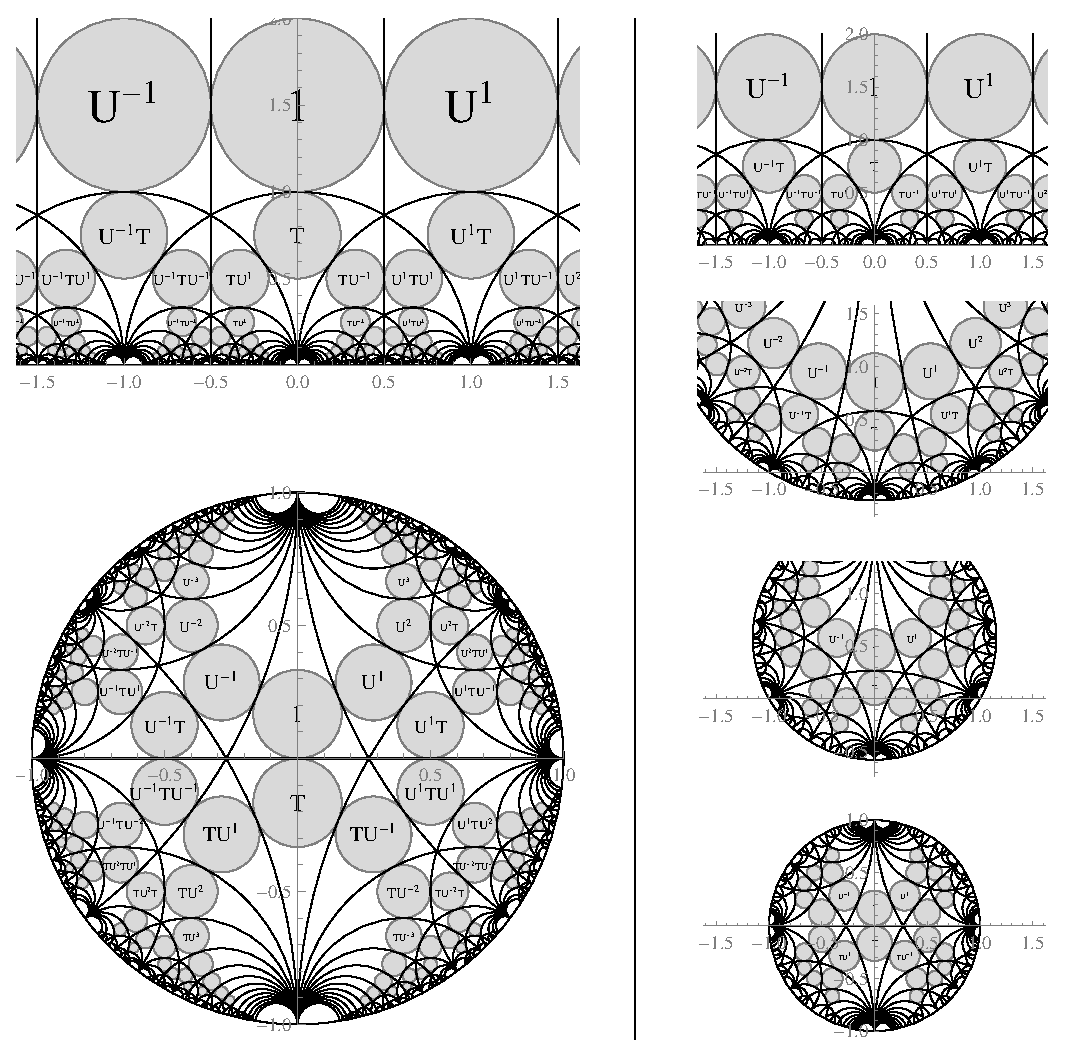
\includegraphics[width=\textwidth]{figures/modular-tiling-1}
\caption{The tessellation of the upper halfplane.}
\label{fig_ModularTiling}
\end{figure}

\begin{figure}
\centering
\includegraphics[width=0.8\textwidth]{figures/modular-tiling-exp-fan}
\caption{The tessellation under the transformation $z \mapsto \exp(2 \pi \ii z)$.}
\label{fig_ModularTilingExpFan}
\end{figure}

\begin{figure}
\centering
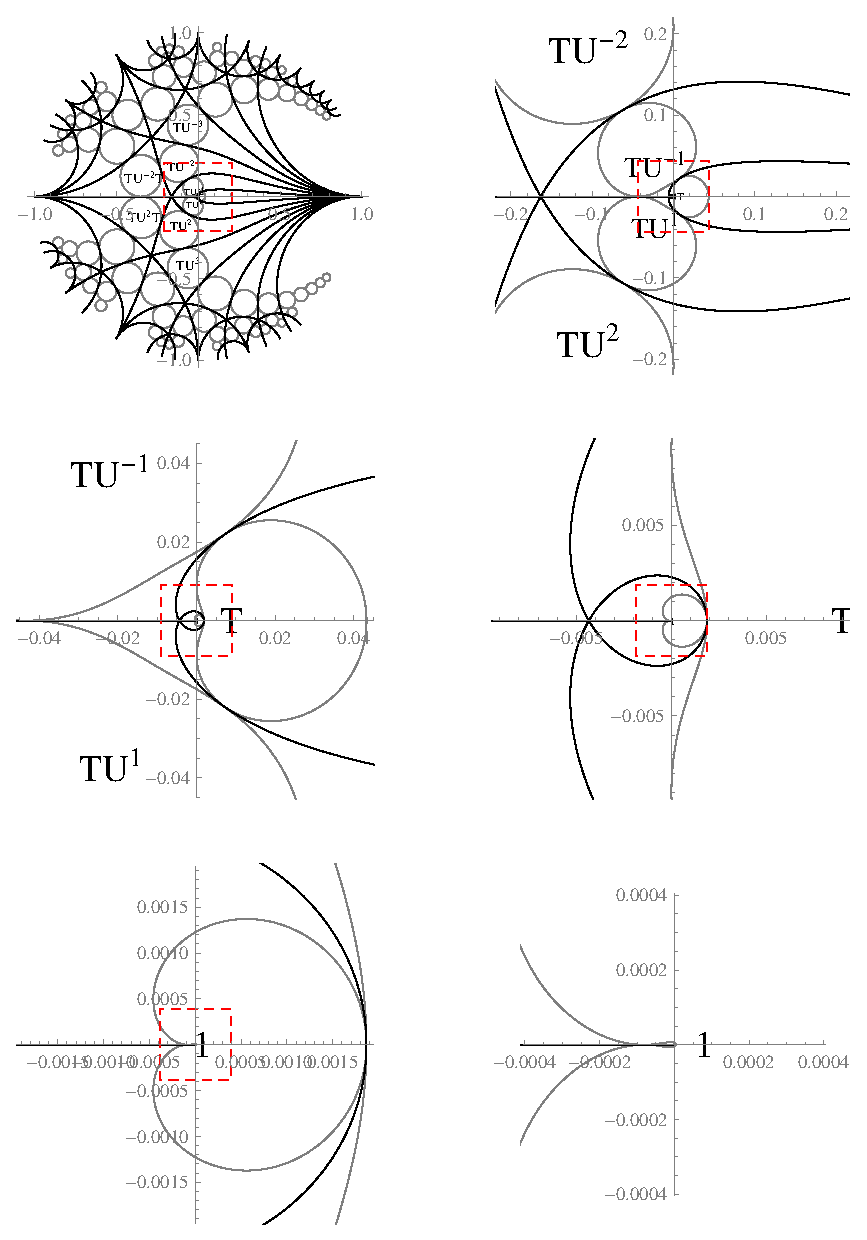
\includegraphics[width=0.8\textwidth]{figures/modular-tiling-exp-zoom}
\caption{The image of the modular tiling under the map $z \mapsto \exp(2 \pi \ii z)$ in the neighborhood of $\infty$.}
\label{fig_ModularTilingExpZoom}
\end{figure}


% ------------------------------------------- Subsection: The action of PSL2(Z)
\subsection{The action of $\PSL{\Z}$ on $\EC$}

In Theorem~\ref{thm_SL2FunDomAlg} we have seen an algorithm which naturally gives rise to a set $\hat{\mathcal{R}} \subseteq \C^2$ which can easily be restricted to a subset $\hat{\FunDom} \subseteq \hat{\mathcal{R}}$ being a fundamental region for the action of $\SL{\Z}$ on $\hat{\mathcal{S}}$. We can exploit this fact in search of a fundamental region for the action on of the (inhomogeneous) modular group $\PSL{\Z}$ on $\EC$. For this purpose we project $\C^2$ onto $\EC$ using the map $\pi : \C^2 \to \EC$,
\begin{equation}
\pi : \cvec{u}{v} \mapsto \frac{u}{v}.
\end{equation}
Let us first consider image of $\hat{\mathcal{S}}$ under $\pi$. If $({}^u_v) \in \hat{\mathcal{S}}$, then by definition $u$ and $v$ are linear independent over $\R$ or linear dependent over $\Q$. In the first case we have $\frac{u}{v} \in \C \setminus \R$ and in the second case $\frac{u}{v} \in \Q \cup \{\infty\}$. This means $\frac{u}{v}$ may be everything but irrational. Denoting set of irrational numbers by $\Irrat = \R \setminus \Q$, we thus have
\begin{equation*}
\pi(\hat{\mathcal{S}}) = \EC \setminus \Irrat.
\end{equation*}
Projection of the set $\hat{\mathcal{R}} \subseteq \C^2$ leads to the region $\mathcal{R} \subseteq \EC$ (see also Figure~\ref{fig_PSL2MinRegion}),
\begin{equation}
\label{eqn_PSL2MinRegion}
\mathcal{R} := \pi\left(\hat{\mathcal{R}}\right) = 
\setdefsz{\Big}{\frac{u}{v} \in \EC}{\abs{u\conj{v} + \conj{u}v} < \min\{\abs{u}^2, \abs{v}^2\}}.
\end{equation}
\begin{figure}
\centering
\includegraphics[width=0.8\textwidth]{figures/minimal-region}
\caption{The region $\mathcal{R} \subseteq \EC$ of numbers $z = u/v \in \EC$ with $\abs{u\conj{v} + \conj{u}v} < \min\{\abs{u}^2,\abs{v}^2\}$. It is obtained by taking the strip $\setdefsz{\big}{z \in \C}{\abs{\Re{z}} < \reci{2}}$  and cutting out two closed disks of unit radius centered about the real points $\pm 1$. The arising vertices are labeled. As usual, $T$ is the transformation $z \mapsto -\reci{z}$ and $\rho = \exp(2 \pi \ii / 3)$ is a third root of unity.}
\label{fig_PSL2MinRegion}
\end{figure}
It follows that $\mathcal{R}$ contains a fundamental region for the action of $\PSL{\Z}$ on $\EC \setminus \Irrat$. As in the homogeneous case, we see from Theorem~\ref{thm_SL2FunDomGlobMin} that equivalence of points within $\mathcal{R}$ can be established only by powers of the transformation $T \in \PSL{\Z}$. Since $T^2 = 1$, in order to obtain a fundamental region we now need to choose for each $z \in \mathcal{R}$ just exactly one of the equivalent points $z$ and $Tz$. This can for example be done such that $\abs{z} > 1$.

\index{Extended upper halfplane}
Note that for understanding the group action of $\PSL{\Z}$ on $\EC \setminus \Irrat$ it is sufficient to look at either the upper or lower halfplane of $\C$, since the group action one halfplane can be easily understood from the group action on the other halfplane, as we trivially have $Az = \conj{A\conj{z}}$. Let us therefore denote by $\mathcal{H}$ the upper halfplane and by $\EU$ the \emph{extended upper halfplane}:
\begin{eqnarray}
\label{eqn_UpperHalfplane}\mathcal{H} &:=& \setdefsz{\big}{z \in \C}{\Im{z} > 0} \\
\label{eqn_ExtUpperHalfplane}
\EU &:=& \mathcal{H} \cup \Q \cup \{\infty\}.
\end{eqnarray}
Clearly $\EU$ is invariant under $\PSL{\Z}$, \ie $\PSL{\Z} \EU = \EU$ and we can also consider $\PSL{\Z}$ acting on $\EU$.

\begin{theorem}
\label{thm_PSL2FunDom}
Let $\mathcal{H}$ and $\EU$ be defined as above. The set
\begin{equation}
\tilde{\FunDom} := \setdefsz{\bigg}{z \in \C}{\abs{\Re{z}} < \reci{2} \text{ and } \abs{z} > 1}
\end{equation}
is a fundamental region for the action of $\PSL{\Z}$ on $\EC \setminus \Irrat$. The part of $\tilde{\FunDom}$ lying in the upper halfplane $\mathcal{H}$, \ie the set
\begin{equation}
\label{eqn_PSL2FunDom}
\FunDom := \tilde{\FunDom} \cap \mathcal{H}
\end{equation}
is a fundamental region for the action of $\PSL{\Z}$ on $\EU$.
\end{theorem}
\begin{proof}
The second statement that $\FunDom = \tilde{\FunDom} \cap \mathcal{H}$ is fundamental region for $\PSL{\Z}$ acting on $\EU$ is a simple consequence of the first statement. For proving that $\tilde{\FunDom}$ is fundamental,  observe that $\tilde{\FunDom}$ is exactly the set
\begin{equation*}
\tilde{\FunDom} = \mathcal{R} \cap \setdef{z \in \C}{\abs{z} > 1},
\end{equation*}
with $\mathcal{R}$ as in (\ref{eqn_PSL2MinRegion}) -- compare also Figure~\ref{fig_PSL2MinRegion}. Obviously $\tilde{\FunDom}$ is a nonempty open subset of $\mathcal{R}$, which is why two distinct points of $\tilde{\FunDom}$ can be equivalent only by the transformation $T$. However, since $\abs{z} > 1$ implies $\abs{Tz} = \abs{-1/z} < 1$, this is impossible. Therefore $\tilde{\FunDom}$ contains no equivalent distinct points.

It remains to show that every $z = \frac{u}{v} \in \mathcal{S}$ is equivalent to a point of the topological closure $\topcl{\tilde{\FunDom}}$ of $\tilde{\FunDom}$. For this purpose apply the algorithm of Theorem~\ref{thm_SL2FunDomAlg} to the vector $({}^u_v) \in \hat{\mathcal{S}}$ in order to obtain a transformation $B \in \PSL{\Z}$ which maps $z$ to a point of $\topcl{\mathcal{R}}$. It then follows that at least one of the points $Bz$ or $TBz$ lies in $\topcl{\tilde{\FunDom}}$.
\end{proof}

We now wish to obtain a \emph{fundamental set} for the action of $\PSL{\Z}$ on $\EU$. For this purpose we need to consider the boundary of $\FunDom$ and to investigate equivalent boundary points and their associated transformations. It turns out that we can define a fundamental set for the action of $\PSL{Z}$ on $\EU$ the following way:

\begin{theorem}[The fundamental set $\FunSet$]
\label{thm_PSL2FunSet}
Denote by $\FunDom$ the fundamental region from (\ref{eqn_PSL2FunDom}). The boundary of $\FunDom$ shall be segmented into the four ``boundary arcs'',
\begin{eqnarray*}
a &:=& \setdefsz{\bigg}{-\reci{2} + y \ii}{y \ge \frac{\sqrt{3}}{2}} \cup \{\infty\},\\
b &:=& \setdefsz{\bigg}{+\reci{2} + y \ii}{y \ge \frac{\sqrt{3}}{2}} \cup \{\infty\},\\
c &:=& \setdefsz{\Big}{\ii \epo{+\ii \phi}}{0 \le \phi \le \frac{\pi}{6}},\\
d &:=& \setdefsz{\Big}{\ii \epo{-\ii \phi}}{0 \le \phi \le \frac{\pi}{6}}.
\end{eqnarray*}
These boundary arcs are mapped onto each other by $Ua = b$ and $Tc = d$. The set
\begin{equation}
\label{eqn_PSL2FunSet}
\FunSet := \FunDom \cup a \cup c
\end{equation}
is a fundamental set for the action of $\PSL{\Z}$ on the extended upper halfplane $\EU$.
\end{theorem}
\begin{proof}
It follows from Theorem~\ref{thm_SL2FunDomGlobMin} that equivalence of boundary points of $\FunDom$ can only be established by transformations $A \in \PSL{Z}$ with $n(A) \le 3$. The full list of candidate transformations therefore comprises of 9 transformations: $T$, $U$, $TU$, $UT$, $TUT$ and the respective inverse transformations (note that $T$ is self-inverse). After looking at these transformations individually, it turns out that in fact only $T$ and $U$ (and $\inv{U}$) map boundary points to boundary points. Indeed $Ua = b$ and $Tc = d$ can readily be seen.
\end{proof}

\begin{remark}
\label{rem_PSL2FunDomGenDisks}
\begin{figure}
\centering
\includegraphics[width=0.8\textwidth]{figures/fundom}
\caption{The fundamental domain $\FunDom$ for the action of the modular group $\PSL{\Z}$ on the extended upper halfplane $\EU$. It is bounded by ``generalized arcs'' $a$, $b$, $c$ and $d$ which correspond to the generalized disks $\mathbb{A}$, $\mathbb{B}$ and the unit disk $\mathbb{D}$. There is a unique disk $\mathcal{I}$ which is tangent $\mathbb{A}$, $\mathbb{B}$ and $\mathbb{D}$.}
\label{fig_PSL2FunDom}
\end{figure}
In Figure~\ref{fig_PSL2FunDom}, we see that the fundamental region $\FunDom$ can also be described in terms of generalized disks (see Definition~\ref{dfn_GenDisk}): With the terminology of Theorem~\ref{thm_PSL2FunSet}, the boundary arcs $a$ and $b$ are indeed ``generalized arcs'' of the closed generalized disks
\begin{equation*}
\mathbb{A} := \mat{0}{1}{1}{1} \quad \text{and} \quad \mathbb{B} := \mat{\phantom{+}0}{-1}{-1}{\phantom{+}1}
\end{equation*}
respectively. The boundary arcs $c$ and $d$ are part of the boundary of the closed unit disk
\begin{equation*}
\mathbb{D} := \mat{1}{\phantom{+}0}{0}{-1}.
\end{equation*}
We see that the fundamental region $\FunDom$ can be characterized as set complement of the union of these three closed g-disks:
\begin{equation*}
\FunDom = \EU \setminus \left(\mathbb{A} \cup \mathbb{B} \cup \mathbb{D}\right).
\end{equation*}
Moreover there exists a unique (open) disk $\mathcal{I} \subseteq \FunDom$, which is tangent to $\mathbb{A}$, $\mathbb{B}$ and $\mathbb{D}$ which we may the \emph{indisk} $\mathcal{I}$ of $\FunDom$.
\end{remark}

The fact that $\FunSet$ is a fundamental set for the action of $\PSL{\Z}$ on $\EU$ can be reformulated as follows: For every point $z \in \EU$ there exists a unique transformation $A \in \PSL{\Z}$ such that $z \in A \FunSet$. In order to determine this transformation, we can adopt the algorithm of Theorem~\ref{thm_SL2FunDomAlg}:

\begin{theorem}[The fundamental set algorithm]
Let $z \in \EU$ be a point of the extended upper halfplane and the fundamental set $\FunSet$ be defined as above. The unique transformation $A$ satisfying $z \in A \FunSet$ can be found by performing the following steps:
\begin{enumerate}
\item Set $j := -1$ and $B_0 := 1$.
\item \label{itm_PSL2FunSetAlgLoop}
Increment $j$ by one and set $z_j := B_j z$. If $z_j \in \FunSet$, then goto step \ref{itm_PSL2FunSetAlgDone}.
\item \label{itm_PSL2FunSetAlgEjDef}
Set $e_j := \floor{\Re{z_j} + \reci{2}}$. 
\item \label{itm_PSL2FunSetAlgNext}
If $z_j - e_j \in \FunSet$, set $B_{j+1} := U^{-e_j}B_j$ -- else set $B_{j+1} := TU^{-e_j}B_j$.
\item Continue with step \ref{itm_PSL2FunSetAlgLoop}.
\item \label{itm_PSL2FunSetAlgDone} 
The desired matrix $A$ is given by $A = \inv{B_j}$.
\end{enumerate}
\end{theorem}
\begin{proof}
Note that the above is essentially a reformulation of the algorithm of Theorem~\ref{thm_SL2FunDomAlg} with the following modifications:
\begin{enumerate}[\quad (a)]
\item The algorithm is reformulated for the inhomogeneous case. The numbers $z_j$ from above and the vectors $x_j$ from the proof of Theorem~\ref{thm_SL2FunDomAlg} correspond by $z_j = \pi(x_j)$.
\item \label{itm_PSL2FunDomAlgModNint}
Instead of using the $\nint{}$ function, we use the above definition  for determining the coefficients $e_j$ -- see step \ref{itm_PSL2FunSetAlgEjDef}. This is to ensure that $z_j - e_j \in [-\reci{2}, \reci{2})$ -- otherwise we would have problems with the termination of the algorithm for the case when some $z_j$ lies on the boundary arc $b$ (as defined in Theorem~\ref{thm_PSL2FunSet}).
\item Theorem~\ref{thm_SL2FunDomAlg} yields a final vector $x_n$ such that $w := \pi(x_n) \in \topcl{\mathcal{R}}$, where $\mathcal{R}$ is defined as in (\ref{eqn_SL2MinRegionDef}). In order to obtain a point in $\FunSet \subseteq \topcl{\mathcal{R}}$, we need to apply to $w$ possibly $T$ and -- if this point lies on the boundary arc $b$ -- possibly $U^{-1}$. We take this into account by explicitly checking whether the application of $T$ in the last iteration of the algorithm is necessary or not (see step \ref{itm_PSL2FunSetAlgNext}) and by the modification discussed in (\ref{itm_PSL2FunDomAlgModNint}).\qedhere
\end{enumerate}
\end{proof}

%Now that we have found a fundamental region and fundamental set, we will investigate how they are mapped by modular transformations. Here it is beneficial to use an alternative description of the fundamental region $\FunDom$ in terms of generalized disks (see Definition~{\ref{dfn_GenDisk}}).  

\begin{figure}
\centering
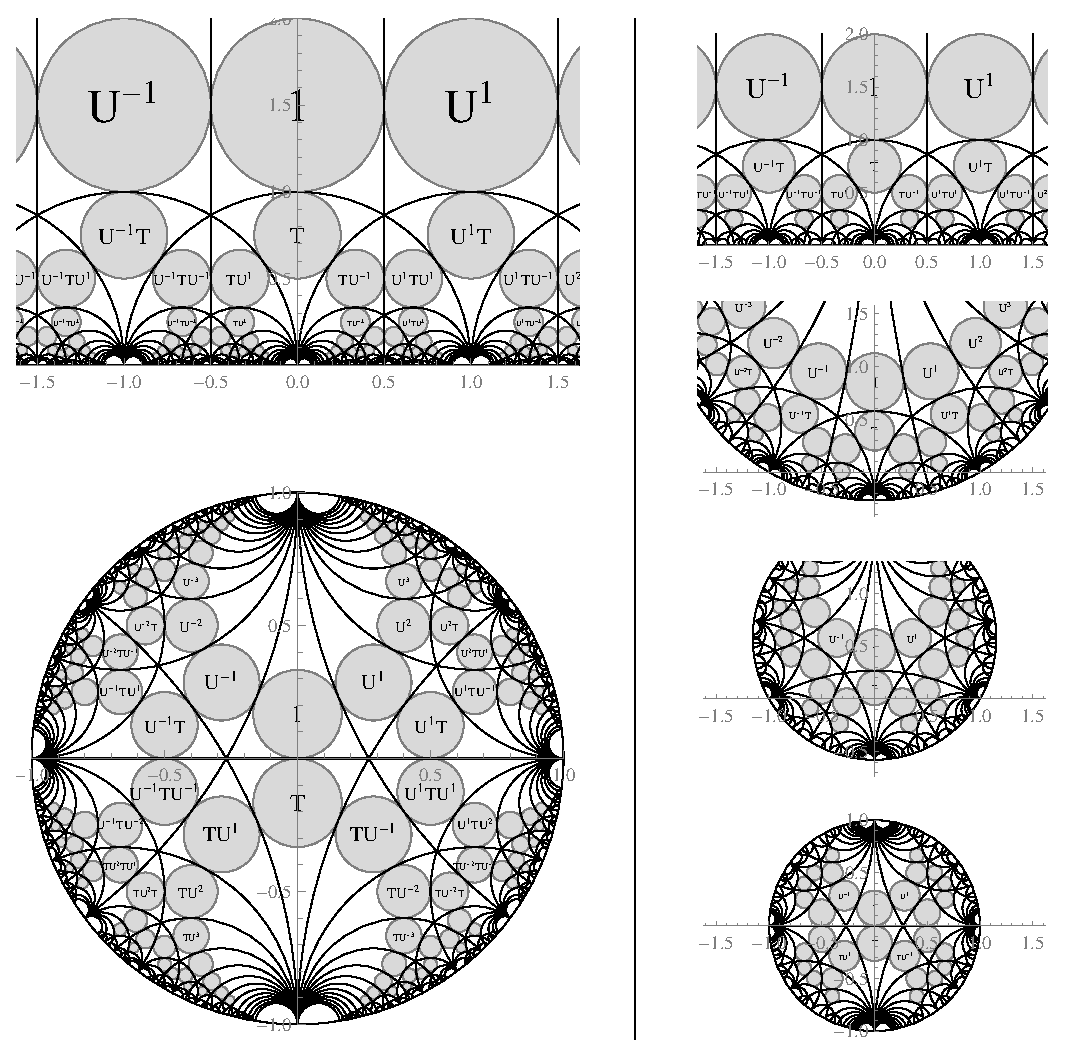
\includegraphics[width=\textwidth]{figures/modular-tiling-1}
\caption{The tessellation of the upper halfplane.}
\label{fig_ModularTiling}
\end{figure}



% ----------------------------------------------------- Section: Modular tiling
\section{The modular tessellation of the upper halfplane}

Since $\FunSet$ is a fundamental set for the action of $\PSL{\Z}$ on $\EU$, its images under all modular transformations cover the extended upper halfplane $\EU$ -- compare also Remark~\ref{rem_FunSetUniqueElement}. Thus for a point $z \in \EU$ there exists a transformation $A \in \PSL{\Z}$ such that $z \in A\FunSet$. We can effectively determine such a transformation by adopting the algorithm of Theorem~\ref{thm_SL2FunDomAlg}:

\begin{theorem}[The fundamental set algorithm]
Let $z \in \EU$ be a point of the extended upper halfplane and let the fundamental set $\FunSet$ be defined as in (\ref{eqn_PSL2FunSet}). A transformation $A$ satisfying $z \in A \FunSet$ can be found by performing the following steps:
\begin{enumerate}
\item Set $j := -1$ and $B_0 := 1$.
\item \label{itm_PSL2FunSetAlgLoop}
Increment $j$ by one and set $z_j := B_j z$. If $z_j \in \FunSet$, then goto step \ref{itm_PSL2FunSetAlgDone}.
\item \label{itm_PSL2FunSetAlgEjDef}
Set $e_j := \floor{\Re{z_j} + \reci{2}}$. 
\item \label{itm_PSL2FunSetAlgNext}
If $z_j - e_j \in \FunSet$, set $B_{j+1} := U^{-e_j}B_j$ -- else set $B_{j+1} := TU^{-e_j}B_j$.
\item Continue with step \ref{itm_PSL2FunSetAlgLoop}.
\item \label{itm_PSL2FunSetAlgDone} 
The desired matrix $A$ is given by $A = \inv{B_j}$.
\end{enumerate}
\end{theorem}
\begin{proof}
Note that the above is essentially a reformulation of the algorithm of Theorem~\ref{thm_SL2FunDomAlg} with the following modifications:
\begin{enumerate}[\quad (a)]
\item The algorithm is reformulated for the inhomogeneous case. The numbers $z_j$ from above and the vectors $x_j$ from the proof of Theorem~\ref{thm_SL2FunDomAlg} correspond by $z_j = \pi(x_j)$.
\item \label{itm_PSL2FunDomAlgModNint}
Instead of using the $\nint{}$ function, we use the above definition  for determining the coefficients $e_j$ -- see step \ref{itm_PSL2FunSetAlgEjDef}. This is to ensure that $z_j - e_j \in [-\reci{2}, \reci{2})$ -- otherwise we would have problems with the termination of the algorithm for the case when some $z_j$ lies on the boundary arc $b$ (as defined in Theorem~\ref{thm_PSL2FunSet}).
\item Theorem~\ref{thm_SL2FunDomAlg} yields a final vector $x_n$ such that $w := \pi(x_n) \in \topcl{\mathcal{R}}$, where $\mathcal{R}$ is defined as in (\ref{eqn_PSL2MinRegion}). In order to obtain a point in $\FunSet \subseteq \topcl{\mathcal{R}}$, we need to apply to $w$ possibly $T$ and -- if this point lies on the boundary arc $b$ -- possibly $U^{-1}$. We take this into account by explicitly checking whether the application of $T$ in the last iteration of the algorithm is necessary or not (see step \ref{itm_PSL2FunSetAlgNext}) and by the modification discussed in (\ref{itm_PSL2FunDomAlgModNint}).\qedhere
\end{enumerate}
\end{proof}

\begin{figure}
\centering
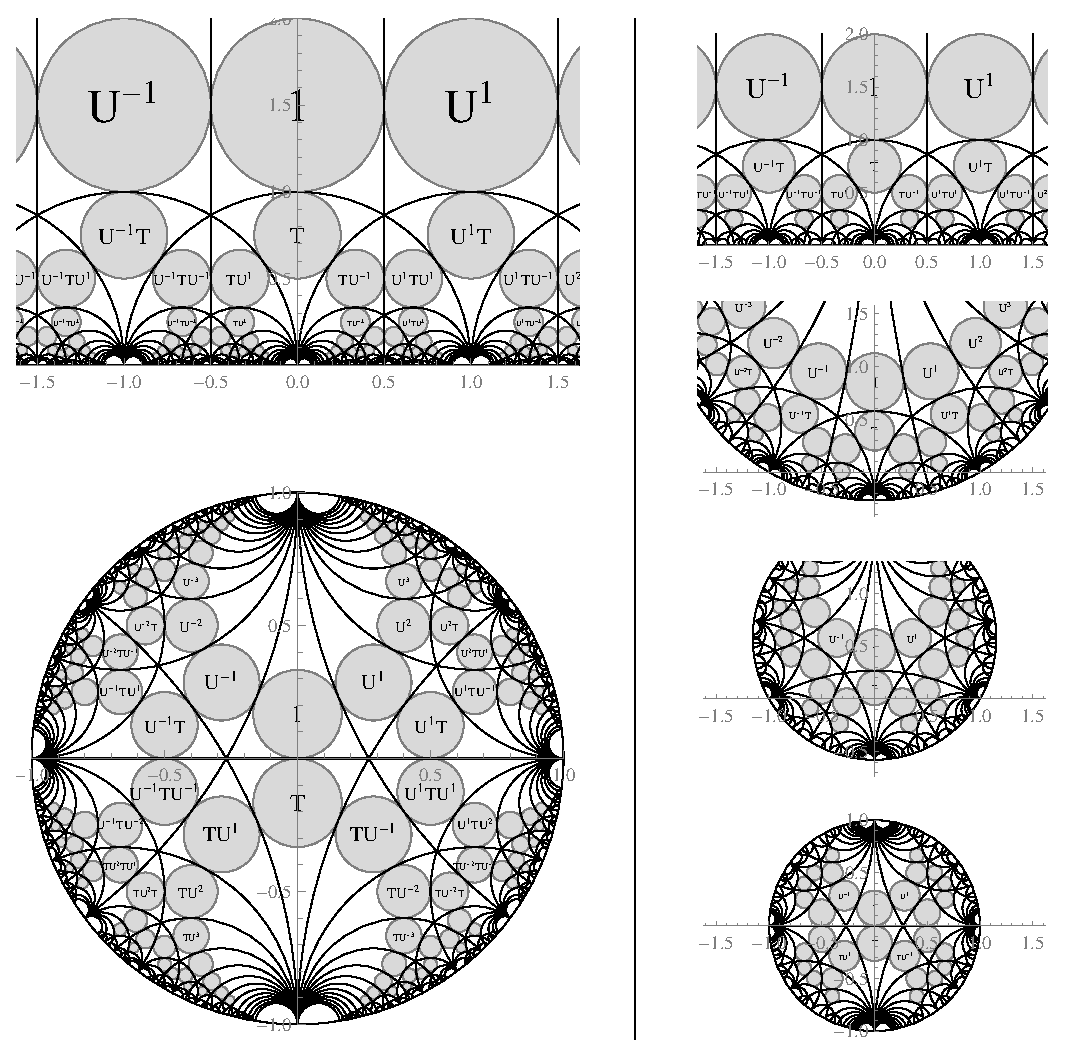
\includegraphics[width=\textwidth]{figures/modular-tiling-1}
\caption{The modular tessellation. The images of $\FunDom$ and $\Indisk$ under all modular transformations (top left) are mapped to the unit circle by the modified Cayley transform $\ModCayley$ (bottom left). A continuous transition between these two images is induced by a quarter-turn of the Riemann sphere and can be seen on the right.}
\label{fig_ModularTiling}
\end{figure}
\index{Tessellation}
\index{Modular!tessellation}
In Figure~\ref{fig_ModularTiling} on the top-left, we see the images of the fundamental region $\FunDom$ and its indisk $\Indisk$ under the transformations of the modular group. Each of these images $A \FunDom$ \resp $A \Indisk$ is labeled by the $T$-$U$ word representation of the corresponding transformation $A \in \PSL{\Z}$. We call this covering of $\EU$ by images of $\FunDom$ the \emph{modular tessellation} of the upper halfplane.

For visualization purposes, the upper halfplane has the obvious disadvantage that we can never see the whole picture. Moreover the true symmetry of the modular tessellation with respect to the transformation $T$ cannot be seen either, but it can be revealed by taking on a different view on the upper halfplane: We have seen in Example~\ref{ex_ModCayleyTransform} that the modified cayley transform $\ModCayley$ maps the upper halfplane to the unit disk. We can therefore use $\ModCayley$ to translate the modular tessellation to the unit disk. This means instead of looking at the regions $A \FunDom$ \resp $A \Indisk$ for all $A \in \SL{\Z}$, we can alternatively depict the regions $\ModCayley A \FunDom$ and the corresponding incircles $\ModCayley A \Indisk$ which is done in the bottom-left picture of Figure~\ref{fig_ModularTiling}. 

For a better understanding of this transformed representation of the modular tessellation, let us identify the drawing area with $\R^2$ rather than with $\C$. Now we note that the point $(0,1)$ corresponds to the point $\infty \in \EU$, the points $(\pm 1, 0)$ relate to $\pm 1 \in \EU$ respectively and the point $(0,-1)$ refers to $0 \in \EU$. The center $(0,0)$ represents the imaginary unit $\ii \in \EU$. In other words, as can be seen in the right column of Figure~\ref{fig_ModularTiling}, $\ModCayley$ bends the real axis to a circle\footnote{In fact, the real axis plus the point $\infty$ can be considered as generalized circle already.}, gluing together its ends at the point $\infty$ and enclosing the upper halfplane in its interior. As we have seen in Example~\ref{ex_ModCayleyTransform}, this continuous transition between the tessellation on the upper halfplane and its image under $\ModCayley$ can be explained by a quarter-turn of the Riemann sphere, compare also Figure~\ref{fig_StereoProjModCayley}.

\begin{remark}
In a more formal context, the bottom-left picture of Figure~\ref{fig_ModularTiling} can also be interpreted in two alternative ways: Firstly, we could consider a different action of $\PSL{\Z}$ on $\EC$, which we may denote as $A \ast z$ for $A \in \PSL{\Z}$ and $z \in \EC$. For its definition we make use of the natural action of the M�bius transformation $\ModCayley A \inv{\ModCayley}$:
\begin{equation*}
A \ast z := (\ModCayley A \inv{\ModCayley}) z.
\end{equation*}
Secondly, we could consider $\EC$ under the natural action of a group $G$ of M�bius transformations which is conjugate to $\PSL{\Z}$:
\begin{equation*}
G := \ModCayley \PSL{\Z} \inv{\ModCayley} = \setdefsz{\Big}{A \in \PSL{\Z[\ii]}}{\htransp{A} = A}.
\end{equation*}
The transformations of $G$ are represented by Hermitian matrices with coefficients in the ring of Gaussian integers $\Z[\ii]$ having determinant 1. Clearly both, the action $\ast$ of $\PSL{\Z}$ as well as the natural action of $G$, leave the unit disk $\ModCayley \mathcal{H}$ invariant. Consequently $\ModCayley \FunDom$ is a fundamental region for both (equivalent) actions on the unit disk. Now the bottom-left picture of Figure~\ref{fig_ModularTiling} can be interpreted as the tessellation induced by either of these two actions with respect to the fundamental region $\ModCayley \FunDom$.
\end{remark}


% ------------------------------------------------ Section: Hyperbolic Geometry
\section{Hyperbolic geometry}

\subsection{Normal polygons and fundamental regions}

%Vonroi diagram

\begin{figure}
\centering
\includegraphics[width=\textwidth]{figures/normpoly-fundom-1}
\caption[The fundamental domain $\FunDom$ as normal polygon]{The fundamental domain $\FunDom$ can alternatively obtained by constructing the normal polygon with respect to any point $z$ on the imaginary axis with $\Im{z} > 1$. Above the point $z = \phi \ii$ (red) has been chosen, where $\phi = \frac{\sqrt{5}+1}{2}$ denotes the golden ratio.}
\label{fig_NormalPolyFunDom}
\end{figure}

\begin{figure}
\centering
\includegraphics[width=\textwidth]{figures/normpoly-fundom-2}
\caption[An alternative fundamental domain for $\PSL{\Z}$]{An alternative fundamental domain for the action of $\PSL{\Z}$ on $\EU$. It is obtained by constructing the normal polygon for the point $\frac{2}{3}(1+\ii)$.}
\label{fig_AltNormalPolyFunDom}
\end{figure}


% --------------------------------------- CHAPTER: ALGORITHMS AND VISUALIZATION
\chapter{Applications in visualization}

\section{The action of modular transformations}

% ------------------------------------------------ Section: Continued fractions
\section{The modular group and continued fractions}

For an arbitrary modular transformation $A$, a representation as product of shifts $U^j: z \mapsto z+j$ and inversions $T: z \mapsto -\reci{z}$ can be found by the $T$-$U$ algorithm of Corollary \ref{cor_ModGrpTUAlg}. By writing out this product, for example in the case when $n=2$, we have
\begin{equation*}
A = U^{e_0}T U^{e_1}T U^{e_2}T U^k,
\end{equation*}
or more explicitly
\begin{equation}
\label{eqn_ALongConFrac}
A(z) = e_0 - \reci{e_1 - \reci{e_2 - \reci{k + z}}}.
\end{equation}
\index{Continued fraction}
\index{Pringsheim notation}
Here a close relation between modular transformations and continued fractions immediately gets apparent. In this section we will investigate this relation somewhat deeper. 
First we will use Pringsheim's more space-saving notation for continued fractions, namely
\begin{equation}
\label{eqn_ConFracNotation}
b_0 + \frac{a_1}{b_1 + \frac{a_2}{b_2 + \frac{a_3}{b_3 + \dots}}} =: 
b_0 + \cfr{a_1}{b_1} + \cfr{a_2}{b_2} + \cfr{a_2}{b_3} + \dots
\end{equation}
In the case when all $a_j = 1$, we adhere to the standard sequence notation for continued fractions:
\begin{equation*}
b_0 + \reci{b_1 + \reci{b_2 + \dots}} =: [b_0,b_1,b_2,\dots].
\end{equation*}
\index{Convergent}
For determining a continued fraction representation for a real number $\alpha$ such that all $a_j = 1$, one usually sets $\alpha_0 := \alpha$ as well as $b_j := \floor{\alpha_j}$ and $\alpha_{j+1} := \reci{\alpha_j - b_j}$ for $j \ge 0$ until some $\alpha_j$ is zero (which is the case if and only if $\alpha \in \Q$). In any way we obtain a finite or infinite sequence of equations 
\begin{equation}
\label{eqn_ConFracEqnSeq}
\alpha = \alpha_0 = b_0 + \reci{\alpha_1}, \quad
\alpha_1 = b_1 + \reci{\alpha_2}, \quad
\alpha_2 = b_2 + \reci{\alpha_3}, \quad \dots
\end{equation}
giving rise to the continued fraction representation $\alpha = [b_0, b_1, b_2, \dots]$. The rational number $c_n := [b_0,b_1,\dots,b_n]$ obtained by truncating the continued fraction representation after the coefficient $b_n$, is called the $n$-th \emph{convergent} of the continued fraction. If the continued fraction is infinte, \ie $\alpha \in \R \setminus \Q$, then we have $\lim_{n \to \infty} c_n = \alpha$.

\begin{remark}
\label{rem_ConFracKinds}
\index{Continued fraction!regular}
Note that by using the method above, all the coefficients $b_j$ with $j > 0$ are positive. A representation for $\alpha$ of this form is called a \emph{regular continued fraction} -- see also \Lehner{}, �9. 

\index{Continued fraction!semi-regular}
In contrast to that, if we set $b_j := \ceil{\alpha_j}$ for some or all of the indices $j$, then also negative coefficients $b_j$, $j > 0$, will occur and we obtain in this way a so called \emph{semi-regular continued fraction} representation of $\alpha$. This is in strong analogy to Remark~\ref{rem_EuclideanAlgorithmRounding} that within the Euclidean algorithm the quotients $q_j$ can be determined by rounding $r_{j-1} / r_j$ either up- or downward. Note that in \Lehner{}, �36, semi-regular continued fractions are defined such that for all $j > 0$ the coefficients $b_j$ are positive, but allowing for $a_j \in \{\pm 1\}$. However this makes no essential difference. 

\index{Continued fraction!canonical}
If we use the nearest integer function in each step, \ie $b_j := \nint{\alpha_j}$ for all $j$, then we have $\abs{b_j} \ge 2$ for all $j > 0$. If additionally $\alpha \in \Q$, then it can be shown that the resulting continued fraction representation is one of minimal length -- according to \Lehner{}, �39, we call finite continued fractions with this minimality property \emph{canonical continued fractions}.
\end{remark}

We can now reformulate Corollary \ref{cor_ModGrpTUAlg} in order to construct a continued fraction representation of any given modular transformation.

\begin{corollary}
\label{cor_ModTransConFrac}
An arbitrary modular transformation $A(z) = \moebius{a}{b}{c}{d}{z}$ can be written as continued fraction
\begin{equation}
\label{eqn_ModTransConFrac}
A(z) = [q_0,q_1,\dots,q_n,(-1)^{n+1}(k+z)]
\end{equation}
where the integers $n$, $q_0,q_1,\dots,q_n$ and $k$ are determined by the algorithm described in Corollary \ref{cor_ModGrpTUAlg}.
\end{corollary}
\begin{proof}
By using the continued fraction representation of $A$ given in (\ref{eqn_ALongConFrac}) and by applying the definition $e_j$ := $(-1)^j q_j$, we see
\begin{IEEEeqnarray}{rCcCcCcCcCcCc}
A(z) &=& e_0 &+& \cfr{-1}{e_1} 
          &+& \cfr{-1}{e_2} 
          &+& \dots 
          &+& \cfr{-1}{e_n} 
          &+& \cfr{-1}{k + z} \nonumber \\
  &=& q_0 &+& \cfr{-1}{-q_1} 
          &+& \cfr{-1}{q_2} 
          &+& \dots 
          &+& \cfr{-1}{(-1)^n q_n} 
          &+& \cfr{-1}{k + z}. \label{eqn_ModTransConFracInterim}
\end{IEEEeqnarray}
Now for every odd $j \le n$ we can rewrite 
\begin{equation*}
\cfr{-1}{-q_j} + \cfr{-1}{\dots} \quad \text{to} \quad \cfr{1}{q_j} + \cfr{1}{\dots}.
\end{equation*}
Thus if $n$ is odd, every numerator $-1$ in (\ref{eqn_ModTransConFracInterim}) can be turned into $+1$. In the other case, when $n$ is even, only one negative numerator at the end, $\frac{-1}{k+z}$, remains, but this can easily be rewritten to $\frac{1}{-(k+z)}$. Taking both cases together, we obtain (\ref{eqn_ModTransConFrac}).
\end{proof}

\begin{remark}
\label{rem_TUAlgConFrac}
It is worth noting that determining a continued fraction representation for a rational number $p/q \in \Q$ with $p,q \in \Z$ is essentially equivalent to applying the Euclidean algorithm to the integers $p$ and $q$: If we set $(r_{-1}, r_0) := (p,q)$ and substitute in (\ref{eqn_ConFracEqnSeq}) $\alpha_j = r_{j-1}/r_j$ for all $j \ge 0$, we obtain
\begin{IEEEeqnarray*}{rClCrCl}
\frac{r_{-1}}{r_0} &=& b_0 + \frac{r_1}{r_0} &\quad\Leftrightarrow\quad& 
  r_{-1} &=& b_0 \cdot r_0 + r_1 \\
\frac{r_0}{r_1} &=& b_1 + \frac{r_2}{r_1} &\Leftrightarrow& 
  r_0 &=& b_1 \cdot r_1 + r_2 \\
\frac{r_1}{r_2} &=& b_1 + \frac{r_3}{r_2} &\Leftrightarrow& 
  r_1 &=& b_2 \cdot r_2 + r_3 \\
 &\vdots& & & &\vdots&
\end{IEEEeqnarray*}
In other words, the coefficients $b_j$ of the desired continued fraction representation are nothing else but the quotients of the Euclidean algorithm which we used to denote by $q_j$.

This observation also allows it to see the $T$-$U$ algorithm of Corollary~\ref{cor_ModGrpTUAlg} in a different light: For a given modular transformation $A(z) = \moebius{a}{b}{c}{d}{z}$, by applying the Euclidean algorithm to $a$ and $c$, we effectively determine a continued fraction representation for the rational number $A(\infty) = \frac{a}{c} = [q_0,q_1,\dots,q_n]$. If we set again $e_j := (-1)^j q_j$, it follows that also the modular transformation $P := U^{e_0}T U^{e_1}T\dots U^{e_n}T$ maps $\infty$ to $\frac{a}{c}$. Since the stabilizer of $\infty$ is generated by the transformation $U$, all transformations with this property can be written as $PU^k$ for some $k \in \Z$.
In particular, if we determine the quotients $q_j$ by rounding to the nearest integer, we obtain a \emph{canonical continued fraction}, \ie a continued fraction representation of minimal length -- compare Remark~\ref{rem_ConFracKinds}. Consequently in this case also the product representation returned by the $T$-$U$ algorithm is of minimal length.
\end{remark}

\begin{corollary}
\label{cor_ConFracModTrans}
Given $r \in \EQ$, a transformation $A \in \PSL{\Z}$ satisfying $A(\infty) = r$ can be found by determining a continued fraction representation of $r$, that is $r = [b_0,b_1,\dots,b_n]$, and setting $A := U^{e_0}T U^{e_1}T \dots U^{e_n}T$ where $e_j := (-1)^j b_j$. In particular, the $k$-th convergent $C_k$, $k \le n$, of this continued fraction representation can be written as $C_k = U^{e_0}T U^{e_1}T \dots U^{e_k}T(\infty)$.
\end{corollary}

We have now seen that there is a natural correspondence between rational numbers, continued fractions and the $T$-$U$ word representations of modular transformations. In order to formalize this correspondence, let us denote by $\Words{\Z} := \bigcup_{n \le 0} \Z^n$ the set of finite integer sequences (or words over the alphabet $\Z$). Furthermore we set $\EQ := \Q \cup \{\infty\}$ and define a map $f: \Words{\Z} \to \EQ$ by
\begin{equation}
\label{eqn_ConFracEvalMap}
\fundef{f}{\Words{\Z}}{\EQ}{(b_0,b_1,\dots,b_n)}{[b_0,b_1,\dots,b_n].}
\end{equation}
Note that evaluation of continued fractions shall take place in $\EQ$ with the natural conventions for treating infinite quantities, \ie for $a \ne 0$ and $b \ne \infty$ we have
\begin{equation*}
\frac{a}{0} = \infty,\quad \frac{b}{\infty} = 0,\quad b \pm \infty = \infty.
\end{equation*}
Moreover the empty continued fraction shall evaluate to $\infty$, \ie $f(\epsilon) = \infty$, where $\epsilon \in \Words{\Z}$ denotes the empty sequence. We call the sequence $\beta \in \Words{\Z}$ a \emph{continued fraction representation} for $f(\beta) \in \EQ$. %Two sequences $\beta, \gamma \in \Words{\Z}$ are defined to be \emph{equivalent}, in symbols $\beta \sim \gamma$, if and only if $f(\beta) = f(\gamma)$. 

Next we set $\Syms := \{T,U\} \subseteq \PSL{\Z}$ and let $\FreeGrp{\Syms}$ be the free group generated by the symbols $T$ and $U$. Moreover we denote by $\langle U \rangle$ the subgroup of $\FreeGrp{\Syms}$ which is generated by the symbol $U$ and the subgroup of $\PSL{\Z}$ generated by the transformation $U$. We now consider left cosets of $\langle U \rangle$ in  $\FreeGrp{\Syms}$ and $\PSL{\Z}$:
\begin{eqnarray*}
\FreeGrp{\Syms} / \langle U \rangle &:=& \setdef{\sigma \langle U \rangle}{\sigma \in \FreeGrp{\Syms}},\\
\PSL{\Z} / \langle U \rangle &:=& \setdef{A \langle U \rangle}{A \in \PSL{\Z}}.
\end{eqnarray*}
It is important to note these are \emph{not} factor groups, as $\langle U \rangle$ is not a normal subgroup of $\PSL{\Z}$ or $\FreeGrp{\Syms}$. In particular, neither $\PSL{\Z} / \langle U \rangle$ nor $\FreeGrp{\Syms} / \langle U \rangle$ carry a ``natural'' group structure -- we will regard them just as sets. 

We now have defined all domains needed for writing $f : \Words{\Z} \to \EQ$ as composition of three other functions, namely $f = g_3 \circ g_2 \circ g_1$, where
\begin{IEEEeqnarray*}{rCcCc}
g_1 &:& \Words{\Z} &\to& \FreeGrp{\Syms} / \langle U \rangle, \\
g_2 &:& \FreeGrp{\Syms} / \langle U \rangle &\to& \PSL{\Z} / \langle U \rangle, \\
g_3 &:& \PSL{\Z} / \langle U \rangle &\to& \EQ.
\end{IEEEeqnarray*}
Let us first turn to the definition of $g_1$, which maps a continued fraction representation to a left coset of a certain $T$-$U$ group word.
\begin{equation}
\label{eqn_MapConFracToPath}
\fundef{g_1}{\Words{\Z}}{\FreeGrp{\Syms} / \langle U \rangle}{(b_0,b_2,\dots,b_n)}{U^{e_0}T U^{e_1}T \dots U^{e_n}T \langle U \rangle} \quad \text{where } e_j := (-1)^j b_j.
%\fundef{g_1}{\Words{\Z}}{\FreeGrp{\Syms} / \langle U \rangle}{(b_0,b_2,\dots,b_n)}{\left( \prod_{j=0}^n (U^{e_j}T) \right) \langle U \rangle} \quad \text{where } e_j := (-1)^j b_j.
\end{equation}
Note that in the case of the empty sequence $\epsilon \in \Words{\Z}$ we have $g_1(\epsilon) = \langle U \rangle$.

In order to define $g_2$, let $\phi: \Sigma \to \PSL{\Z}$ be the canonical embedding, \ie $\phi(T) = T$ and $\phi(U) = U$. Let $\overline{\phi}$ be the unique extension of $\phi$ to a homomorphism $\FreeGrp{\Syms} \to \PSL{\Z}$, according to Theorem~\ref{thm_FreeGrpUniqueHom}. Note that $\overline{\phi}$ is just the map which evaluates $T$-$U$ group words to concrete elements of $\PSL{\Z}$ in the obvious way. The function $g_2$ now takes  a left coset in $\FreeGrp{\Syms}$ to a left coset in $\PSL{\Z}$ by
\begin{equation}
\label{eqn_MapPathToCoset}
\fundef{g_2}{\FreeGrp{\Syms} / \langle U \rangle}{\PSL{\Z} / \langle U \rangle}{\sigma \langle U \rangle}{\overline{\phi}(\sigma) \langle U \rangle.}
\end{equation}
Last but not least we define $g_3$ as the map which evaluates the transformations of a left coset $A \langle U \rangle \in \PSL{\Z} / \langle U \rangle$ at the point $\infty$. Note that the result is the same for all transformations within one coset because $\langle U \rangle$ is exactly the stabilizer of $\infty$, \ie $\langle U \rangle = \setdef{B \in \PSL{\Z}}{B(\infty) = \infty}$. This allows us to define
\begin{equation}
\label{eqn_MapCosetToEQ}
\fundef{g_3}{\PSL{\Z} / \langle U \rangle}{\EQ}{A \langle U \rangle}{A(\infty).}
\end{equation}

\begin{lemma}
\label{lem_ConFracMapEquality}
The maps $g_1$, $g_2$, $g_3$ and $f$, defined as above, satisfy
\begin{equation*}
f = g_3 \circ g_2 \circ g_1.
\end{equation*}
\end{lemma}
\begin{proof}
It follows from Corollary~\ref{cor_ConFracModTrans} that the composed map $g_2 \circ g_1: \Words{\Z} \to \PSL{\Z} / \langle U \rangle$ takes a continued fraction representation $(b_0,b_1,\dots,b_n)$ to a left coset $A \langle U \rangle$, such that $g_3(A \langle U \rangle) = A(\infty) = [b_0,b_1,\dots,b_n]$. Therefore we have indeed $f = g_3 \circ g_2 \circ g_1$.
\end{proof}

\begin{lemma}
\label{lem_MapConFracToPathInjective}
The map $g_1$ defined in (\ref{eqn_MapConFracToPath}) is injective. Its image $g_1(\Words{\Z})$ consists precisely of those cosets $\sigma \langle U \rangle \in \FreeGrp{\Syms} / \langle U \rangle$, where the $T$-$U$ group word $\sigma$ is such that:
\begin{enumerate}[\quad(i)]
\item \label{itm_NotContainsTInv}
The reduced form of $\sigma$ never contains the symbol $\inv{T}$.
\item \label{itm_RightmostIsT}
If the reduced form of $\sigma$ is not empty, its rightmost symbol is $T$.
\end{enumerate}
In particular there is a one-to-one correspondence between all continued fraction representations and $T$-$U$ group words of this form. 
\end{lemma}
\begin{proof}
The fact that $g_1$ is injective is obvious. It is also clear that the word
\begin{equation}
\label{eqn_ConFracTUWord}
U^{e_0}T U^{e_1}T \dots U^{e_n} T
\end{equation}
with $n \ge 0$, $e_j \in \Z$ occurring in the definition of $g_1$ already is in  reduced form and satisfies the conditions (\ref{itm_NotContainsTInv}) and (\ref{itm_RightmostIsT}). Conversely, every reduced word $w$ satisfying (\ref{itm_NotContainsTInv}) and (\ref{itm_RightmostIsT}) has necessarily the form
\begin{equation*}
w = U^{k_1} T^{\ell_1} U^{k_2} T^{\ell_2} \dots U^{k_m} T^{\ell_m},
\end{equation*}
with $m >= 0$, $k_j \in \Z$ and $\ell_j \ge 1$. Because for $k \ge 1$, $T^k$ and $(TU^0)^{k-1}T$ are \emph{identical} as words, we can for sure notate $w$ alternatively in the form (\ref{eqn_ConFracTUWord}).
\end{proof}

\begin{lemma}
\label{lem_MapCosetToEQBijective}
The map $g_3$ defined in (\ref{eqn_MapCosetToEQ}) is bijective. In particular there is a one-to-one correspondence between the left cosets of $\langle U \rangle$ in $\PSL{\Z}$ and the extended rational numbers $\EQ$.
\end{lemma}
\begin{proof}
If $g_3(A \langle U \rangle) = g_3(B \langle U \rangle)$, then $A(\infty) = B (\infty)$. This is equivalent to $\inv{B}A \in \langle U \rangle$ or $A \langle U \rangle = B \langle U \rangle$. Therefore $g_3$ is injective. Since $f = g_3 \circ g_2 \circ g_1$ is surjective, the same must be true for $g_3$.
\end{proof}

\begin{figure}
\centering
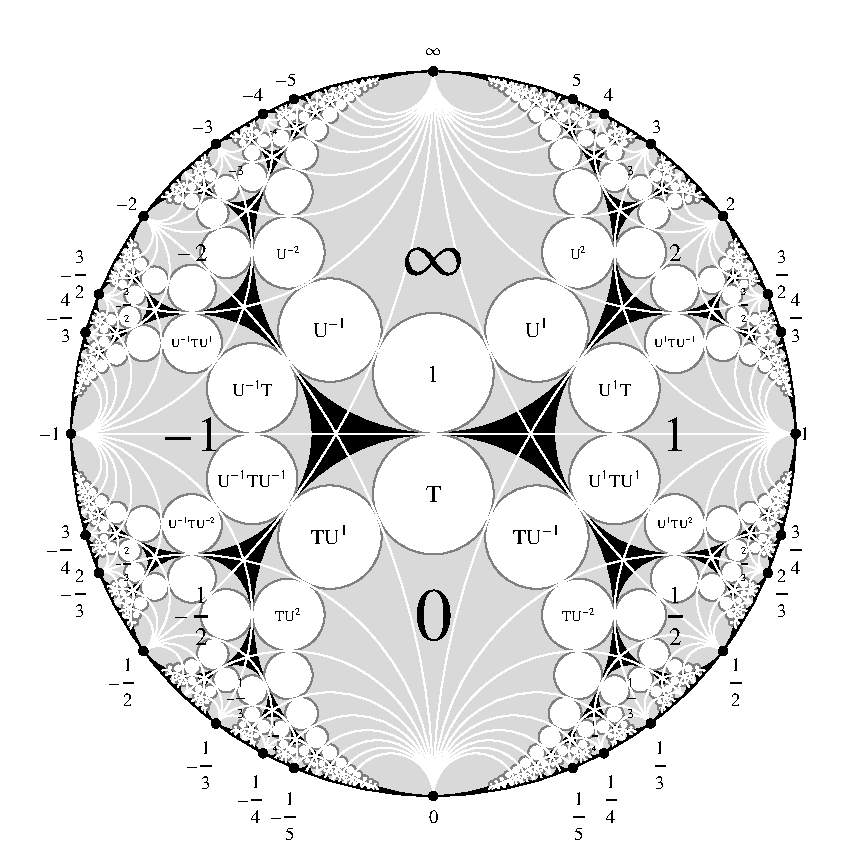
\includegraphics[width=\textwidth]{figures/ford-disks}
\caption{The modular tessellation under the modified Cayley transform $\ModCayley$. The Ford disk $\Forddisk_\infty$ (light gray, labeled with ``$\infty$'') encloses precisely the indisks $B\Indisk$, $B \in \langle U \rangle$, in its interior. It can thus be considered as representative for the subgroup $\langle U \rangle$ in $\PSL{\Z}$. The images of $\Forddisk_\infty$ under the modular group are all Ford disks $\Forddisk_r$ with $r \in \EQ$. For $A \in \PSL{\Z}$, we have $A\Forddisk_\infty = \Forddisk_r$ exactly when $A(\infty) = r$. Therefore $\Forddisk_r$ corresponds directly to both, the  number $r$ (the point, where $\Forddisk_r$ touches the extended real axis) and the left coset $A\langle U \rangle$ ($\Forddisk_r$ encloses precisely the indisks $B\Indisk$, $B \in A \langle U \rangle$).}
\label{fig_FordDisks}
\end{figure}
Looking at the modular tessellation, Figure~\ref{fig_ModularTiling}, we see that the images of the indisk $\Indisk$ of the fundamental region $\FunDom$ 
have a natural one-to-one correspondence to modular transformations, \ie the disk $A\Indisk$ can be considered as a graphical representative for the modular transformation $A$. The question arises, if there is such a visual and clear representation also for left cosets of $\langle U \rangle$ in $\PSL{\Z}$. Indeed, we can see in Figure~\ref{fig_FordDisks} -- depicting the modular tessellation under the modified Cayley transform $\ModCayley$ -- that the disks $U^k\Indisk$, $k \in \Z$ form a ``generalized ring'' which asymptotically approaches the point $\infty$. We can enclose this ring in a generalized disk -- in Figure~\ref{fig_FordDisks}, this enclosing disk is shown in light gray and is labeled with ``$\infty$''.
\begin{definition}
\label{dfn_FordDisk}
\index{Ford disk}
The unique (open) g-disk $\Forddisk_\infty$ containing all the disks $U^k\Indisk$, $k \in \Z$, in its interior and being tangent to each of them is called the \emph{Ford disk at $\infty$}. It contains all points $z \in \C$ with $\Im{z} > 1$. Its defining matrix is given by
\begin{equation}
\label{eqn_FordDisk}
\Forddisk_\infty = \mat{0}{-\ii}{\ii}{2}.
\end{equation}
For a modular transformation $A = \smallmat{a}{b}{c}{d} \in \PSL{\Z}$, the image of $\Forddisk_\infty$ under $A$ is called the \emph{Ford disk at $\frac{a}{c}$}, $\Forddisk_{\frac{a}{c}} := A\Forddisk_\infty$.
\end{definition}

The above definition as well as the bijective correspondence between left cosets of $\langle U \rangle$ in $\PSL{\Z}$ and the extended rational numbers $\EQ$ (Lemma~\ref{lem_MapCosetToEQBijective}) can now be explained in view of Figure~\ref{fig_FordDisks}: We can see that every Ford disk $\Forddisk_r$ (the light gray disks, each of them labeled with the corresponding number $r \in \EQ$), ``touches'' the extended real axis $\R_\infty := \R \cup \{\infty\}$ (appearing as unit circle under the modified Cayley transform) exactly in the point $r$, that is
\begin{equation*}
\topcl{\Forddisk_r} \cap \R_\infty = \{r\} \quad \text{for all } r \in \EQ.
\end{equation*}
For the seeing the relation of Ford disks to left costets of $\langle U \rangle$ in $\PSL{\Z}$, first observe that the Ford disk $\Forddisk_\infty$ encloses precisely all indisks $B \Indisk$, $B \in \langle U \rangle$. In this sense, we can consider $\Forddisk_\infty$ as a graphical representative for the subgroup $\langle U \rangle$ of $\PSL{\Z}$. Clearly every Ford disk $\Forddisk_r$, $r \in \EQ$, is the image of $\Forddisk_\infty$ under some transformation $A \in \PSL{\Z}$, \ie $A\Forddisk_\infty = \Forddisk_r$, which is the case if and only if $A(\infty) = r$. Consequently $\Forddisk_r$ encloses all indisks $B\Indisk$, $B \in A \langle U \rangle$ and thus can be considered as graphical representative for the coset $A \langle U \rangle$.

Also the statement of Lemma~\ref{lem_MapConFracToPathInjective}, the one-to-one correspondence between continued fraction representations and $T$-$U$ words of the form (\ref{eqn_ConFracTUWord}), has a nice visual interpretation, as we will illustrate in the following example.

\begin{figure}
\centering
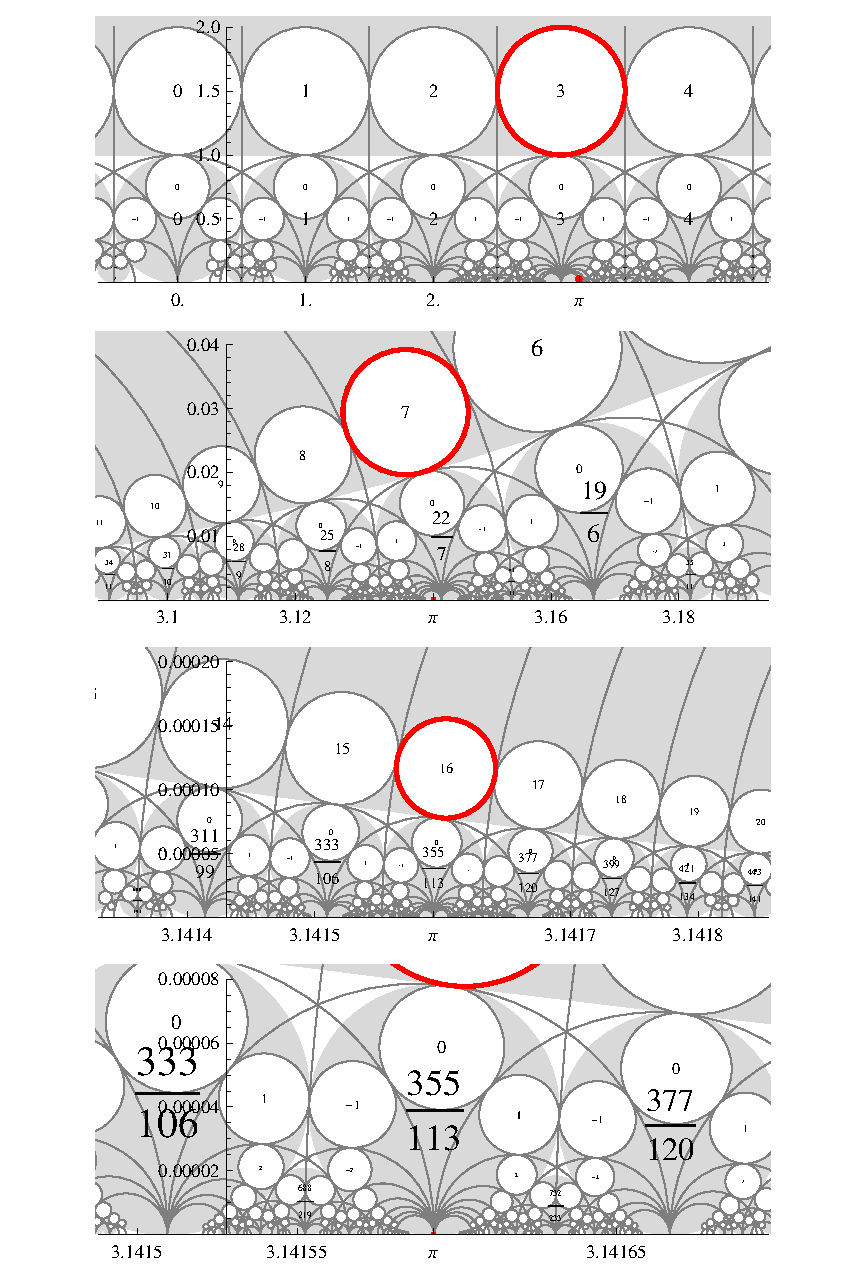
\includegraphics[width=\textwidth]{figures/cont-frac-pi}
\caption{$\pi = \frac{355}{113}$ -- well, almost.}
\label{fig_ConFracPi}
\end{figure}
\begin{example}
\label{ex_ConFracPi}
Consider the (semi-regular) continued fraction expansion of the irrational number $\pi$, obtained by using the nearest integer function for rounding the $\alpha_j$ -- compare Remark~\ref{rem_ConFracKinds}. The first few coefficients of this continued fraction are given by
\begin{equation*}
\pi = [3, 7, 16, -294, 3, -4, 5, -15, -3, 2, 2, 2, 2, 3, -85, -3, 2, 15, 3, 14,\dots]
\end{equation*}
More coefficients can be found by looking up the sequence A133593 at the \emph{On-Line Encyclopedia of Integer Sequences (OEIS)}\footnote{https://oeis.org}. By Corollary~\ref{cor_ConFracModTrans}, the convergents of this continued fraction give rise to a sequence of Modular transformations:
\begin{IEEEeqnarray*}{rCcCl}
\lbrack 3 \rbrack &=& 3
  &=& U^3 T (\infty),\\
\lbrack 3,7 \rbrack &=& \frac{22}{7} 
  &=& U^3 T U^{-7} T (\infty),\\
\lbrack 3,7,16 \rbrack &=& \frac{355}{113}
  &=& U^3 T U^{-7} T U^{16} T (\infty),\\
\lbrack 3,7,16,-294 \rbrack &=& \frac{104348}{33215} 
  &=& U^3 T U^{-7} T U^{16} T U^{294} T (\infty),\\
&\vdots& &\vdots&
\end{IEEEeqnarray*}
The $T$-$U$ words occurring in this sequence can now be interpreted as ``path'' through the set of indisks $A\Indisk$, $A \in \PSL{\Z}$ as follows:
\begin{enumerate}
\item Start with the Ford disk $\Forddisk_\infty$. Label each indisk $U^k\Indisk$ (contained in $\Forddisk_\infty$) with the corresponding integer $k \in \Z$. The Ford disk $U^3 T \Forddisk_\infty = \Forddisk_3$, corresponding to the convergent $c_0 = 3$, can be approached by starting at the indisk $\Indisk$ (carrying the label 0), going 3 steps right to the indisk with label 3, $U^3 \Indisk$ (marked red in the first row of Figure~\ref{fig_ConFracPi}) and finally applying $T$, that is going from there to the tangent indisk $U^3 T \Indisk$, lying within the Ford disk $\Forddisk_3$.
\item For convenience, set $A_1 := U^3 T$. Within the Ford disk $\Forddisk_3$, label each indisk $A_1 U^k \Indisk$ with the \emph{negated}\footnote{The negation of the sign comes from the fact that we want the indisk labels to correspond to the coefficients $b_j$ of the continued fraction rather than to the exponents $e_j = (-1)^j b_j$ of the $T$-$U$ word.} integer $-k$. Go from indisk $A_1 \Indisk$ (labeled 0) seven steps to the indisk with label 7, $A_1 U^{-7}\Indisk$ -- see second row of Figure~\ref{fig_ConFracPi}. Applying $T$ again takes us to the indisk $A_1 U^{-7} T \Indisk$ within the Ford disk corresponding to the next convergent of the continued fraction: $\Forddisk_{c_1}$, $c_1 = \frac{22}{7}$.
\item Set $A_2 := U^3 T U^{-7} T$. As above, label all indisks $A_2 U^k \Indisk$ within $\Forddisk_{c_1}$ with $k$ and go from $A_2 \Indisk$ with label 0 sixteen steps to $A_2 U^{16} \Indisk$ with label 16 (Figure~\ref{fig_ConFracPi}, 3rd row) and from there to $A_2 U^{16} T \Indisk$, lying within $\Forddisk_{c_2}$, $c_2 = \frac{355}{113}$.

\dots
\end{enumerate}
\end{example}

Without explicating further steps of the above example, we can easily imagine how this generalizes to different continued fraction representations of arbitrary real numbers: Given a continued fraction $\alpha = [b_0,b_1,\dots]$, we start with the indisk $\Indisk^{(0)} := \Indisk$ contained in the Ford disk $\Forddisk^{(0)} := \Forddisk_\infty$. For every $j \ge 0$, we label the indisks contained in $\Forddisk^{(j)}$ with successive integers in counter-clockwise direction (if $j$ is even) or in clockwise direction (if $j$ is odd) in such a way that the disk $\Indisk^{(j)}$ carries the label 0. Now we choose $\Indisk^{(j+1)}$ as the unique indisk which is exterior to $\Forddisk^{(j)}$ and tangent to the disk with label $b_j$ (within $\Forddisk^{(j)}$). Moreover we choose as $\Forddisk^{(j+1)}$ the unique Ford disk containing $\Indisk^{(j+1)}$. 

\index{Indisk!path}
Considering also ``intermediate'' indisks (those with labels between 0 and $b_j$ within $\Forddisk^{(j)}$), we describe in this way an \emph{indisk-path}, or in other words a chain of successively tangent disks, through the set of all indisks $A\Indisk$, $A \in \PSL{\Z}$. Such a path always starts at $\Indisk$ and ends at some $U^{e_0}T U^{e_1}T \dots U^{e_n}T\Indisk$, appending exactly one symbol $U$, $\inv{U}$ or $T$ to the previous group word when moving one step forward along the path. Obviously these paths can be considered as a visual representation of $T$-$U$ words of the form (\ref{eqn_ConFracTUWord}) and we can draw the following conclusions:
\begin{itemize}
\item All different paths starting at $\Indisk$ and ending within a given Ford disk $\Forddisk_r$ give rise to different continued fraction representations of the same rational number $r \in \EQ$. In particular continued fraction representations are not unique in any way (unless we impose certain conditions on its coefficients $b_j$, as for example regularity -- compare \Lehner{}, �9).
\end{itemize}

\todo{19}{The modular group and ford circles}


% ------------------------- Section: Modular tiling, exponential transformation
\section{The modular tessellation and the exponential transformation}

\begin{figure}
\centering
\includegraphics[width=0.8\textwidth]{figures/modular-tiling-exp-fan}
\caption{The tessellation under the transformation $z \mapsto \exp(2 \pi \ii z)$.}
\label{fig_ModularTilingExpFan}
\end{figure}

\begin{figure}
\centering
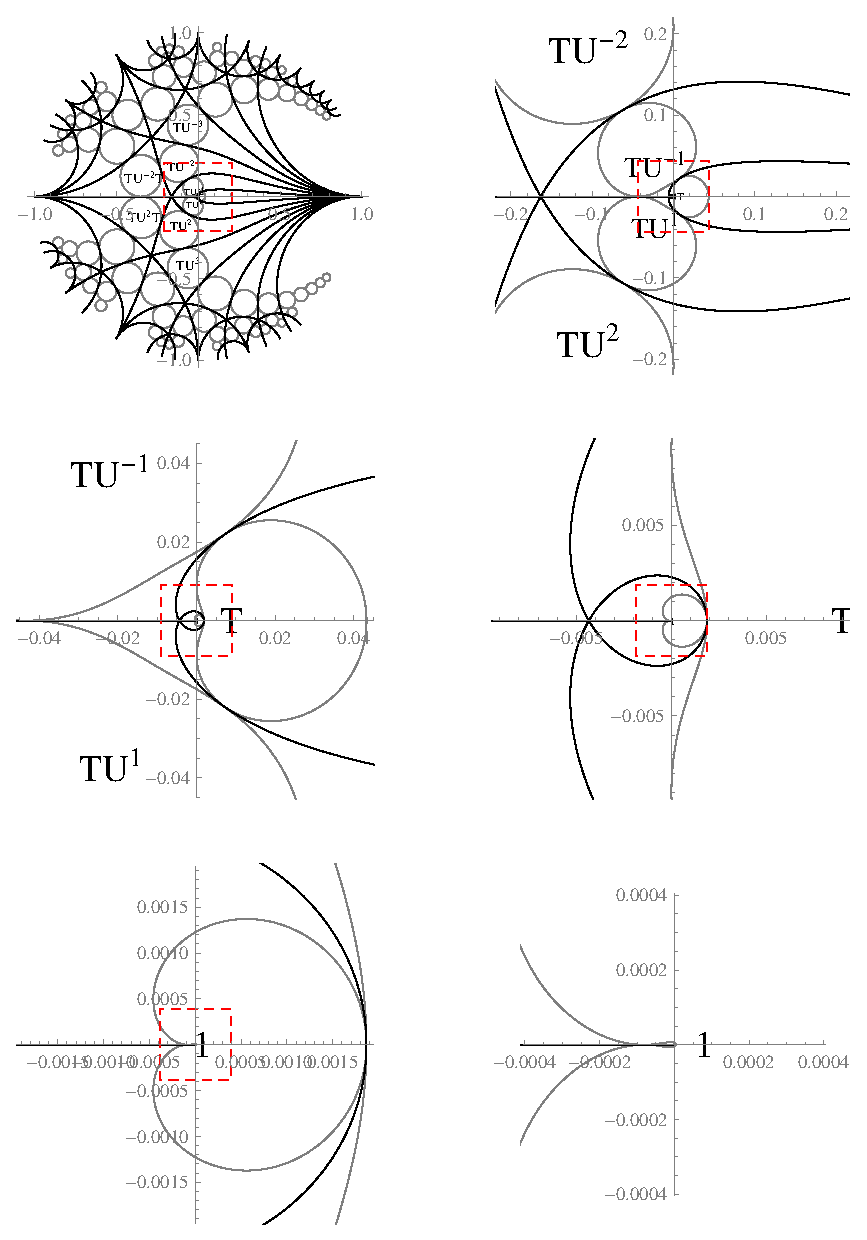
\includegraphics[width=0.8\textwidth]{figures/modular-tiling-exp-zoom}
\caption{The image of the modular tiling under the map $z \mapsto \exp(2 \pi \ii z)$ in the neighborhood of $\infty$.}
\label{fig_ModularTilingExpZoom}
\end{figure}


% -------------------------------------------------- Section: Klein j invariant
\section{Modular functions}

We devote the last section of this thesis to the visualization of modular functions. The theory of modular functions is a branch of complex analysis whose importance and beauty lies most notably in its connections to number theory. We will however not dive deeply into this theory. Instead we will content ourselves with depicting graphs of certain selected modular functions, enjoying their visual aesthetics and reading off some of its properties, like zeros and poles as well as their order. Unfortunately such illustrations of modular functions are rarely found in literature. Therefore this section should be considered as complementary material to more comprehensive treatments of modular functions given for example in \Klein{}, \Lehner{} or \Schoeneberg{}.

\index{Meromorphic function}
Modular functions are meromorphic maps (\ie maps which are holomorphic\footnote{Holomorphic functions are also frequently called ``analytic''.} except for isolated poles, or in other words, maps which can be represented as quotient of two holomorphic functions) which are defined on the upper half-plane and which are invariant under the transformations of the modular group.

\begin{definition}[Modular function]
Let the upper halfplane $\mathcal{H}$ and the extended upper halfplane $\EU$ be defined as in (\ref{eqn_Upperhalfplane}) and (\ref{eqn_ExtUpperhalfplane}) respectively.
A map $f : \EU \to \EC$ is called a \emph{modular function}, if it satisfies the following conditions:
\begin{enumerate}[\quad(i)]
\item $f$ is meromorphic on the upper half-plane $\mathcal{H}$.
\item On $\EU$ we have $f = f \circ A$ for all $A \in \PSL{\Z}$.
\item There is a constant $C \ge 0$ such that $f$ has a series expansion of the form
\begin{equation*}
f(z) = \sum_{k \ge k_0} a_k \exp(2 \pi \ii k z),
\end{equation*}
with $k_0 \in \Z$, $a_k \in \C$, $a_{k_0} \ne 0$, which converges for all $z \in \mathcal{H}$ with $\Im{z} > C$. Moreover, 
\begin{equation*}
f(\infty) = \begin{cases}
0 & \text{if } k_0 > 0,\\
a_0 & \text{if } k_0 = 0,\\
\infty & \text{if } k_0 < 0.
\end{cases}
\end{equation*}
\end{enumerate}
\end{definition}

\begin{remark}For the proof that modular functions indeed exist we refer to \Schoeneberg{}, Chapter II, �3.
\end{remark}

\index{Absolute modular invariant}
\index{Klein's complete invariant}
A modular function of essential importance is the $J$ function, also known as the \emph{absolute modular invariant} or \emph{Klein's complete invariant}. One of its important properties is, that on the fundamental domain $\FunDom$ it takes on each value in $\EC$ exactly once. In other words, $J$ can be considered as bijective map from $\FunDom$ to $\EC$. 

In order to discuss this one-to-one mapping between $\FunDom$ and $\EC$ under $J$, let us denote the boundary arcs of $\FunDom$ again by $a,b,c$ and $d$, as in Figure~\ref{fig_PSL2FunDom}. Moreover, denote by $e := \setdef{\lambda \ii}{\lambda \ge 1} \cup \{\infty\}$ the arc which splits $\FunDom$ into two symmetric havles, \ie two open connected components. Let us denote these open sets by $\FunDom_\text{left}$ and $\FunDom_\text{right}$ respectively. For the special boundary points $\ii$, $\rho$ and $\infty$ we have
\begin{equation*}
J(\ii) = 1, \quad J(\rho) = 0, \quad J(\infty) = \infty.
\end{equation*}
Moreover, the following mappings of sets are all injective:
\begin{itemize}
\item The left boundary arc $a$ and the right boundary arc $b$ of $\FunDom$ are both mapped to the set $\overline{\R}_{\le 0} := \setdef{z \in \R}{z \le 0} \cup \{\infty\}$:
\begin{equation*}
J(a) = J(b) = \overline{\R}_{\le 0}.
\end{equation*}
\item The boundary arcs $c$ and $d$ of $\FunDom$ are both mapped to the interval $[0,1]$:
\begin{equation*}
J(c) = J(d) = [0,1].
\end{equation*}
\item The ``symmetry arc'' $e$ is mapped to $\overline{\R}_{\ge 1} := \setdef{z \in \R}{z \ge 1} \cup \{\infty\}$:
\begin{equation*}
J(e) = \overline{\R}_{\ge 1}. 
\end{equation*}
\end{itemize}
In particular, the boundaries of $\FunDom_\text{left}$ and $\FunDom_\text{right}$ are both injectively mapped to $\R \cup \{\infty\}$. 
Finally, the images of $\FunDom_\text{left}$ and $\FunDom_\text{right}$ under $J$ are exactly the upper and lower half-plane:
\begin{equation*}
J(\FunDom_\text{left}) = \mathcal{H} \quad\text{and}\quad
J(\FunDom_\text{right}) = -\mathcal{H}.
\end{equation*}

Unfortunately, plotting the function graph of $J$, or more generally the function graph of any map $f: \EC \to \EC$ is not directly possible, as it is in fact a 4-dimensional object.\footnote{It involves two dimensions for real and imaginary part of the function argument and two more dimensions for real and imaginary part of the function value.} However there is a simple idea for getting around this problem: We assign each $z \in \EC$ a certain color $\col{z}$ and obtain a picture of $f$ by dying each point $z$ on the complex plane in the color $\col{f(z)}$. Our choice of the color coding is quite simple: 
\begin{itemize}
\item The tone of the color $\col{z}$ encodes the complex argument of $z$:\\
\begin{tabular}{rlccccc}
Red &($\arg{z} = 0$) &$\to$& Orange &$\to$& Yellow &$\to$ \\
Green &($\arg{z} = \half{\pi}$) &$\to$& Turquoise &$\to$ \\
Cyan &($\arg{z} = \pi$) &$\to$& Blue &$\to$\\
Violet &($\arg{z} = -\half{\pi}$) &$\to$& Magenta &$\to$& Red (again).
\end{tabular}
\item The saturation and brightness of the color $\col{z}$ encodes the absolute value of $z$. For this purpose, we use the continuous map 
\begin{equation*}
b(r) := \begin{cases}
0 & \text{if } r = 0,\\
\reci{\pi}\arctan(\ln r)  + \reci{2} & \text{if } r \in (0,\infty),\\
1 & \text{if } r = \infty
\end{cases}
\end{equation*}
to first bring $\abs{z}$ to the interval $[0,1]$. Then we define the saturation of $\col{z}$ as $1 - b(\abs{z})^2$ and its brightness as $1 - (1 - b(\abs{z})^2)$. This means that $\col{z}$ changes gradually from a perfect black (if $z = 0$) to a perfect white ($z = \infty$) as absolute value of $z$ grows.
\end{itemize}
\begin{figure}
\centering
\includegraphics[width=0.8\textwidth]{figures/klein-j}
\caption{The composition of the Klein modular invariant function and the inverse modified Cayley transform $j \circ \inv{\ModCayley}$.}
\label{fig_KleinJ}
\end{figure}


\begin{figure}
\centering
\begin{tabular}{c c c}
\includegraphics[width=0.45\textwidth]{figures/klein-jinv} & \quad &
\includegraphics[width=0.45\textwidth]{figures/klein-jm1} \\
\\
\includegraphics[width=0.45\textwidth]{figures/klein-jsqr} & \quad &
\includegraphics[width=0.45\textwidth]{figures/klein-j-mod-cayley}
\end{tabular}
\caption{The composition of the Klein modular invariant function and the inverse modified Cayley transform $j \circ \inv{\ModCayley}$.}
\label{fig_FunctionsOfJ}
\end{figure}

\begin{figure}
\centering
\includegraphics[width=0.8\textwidth]{figures/klein-jfib-large}
\caption{The composition of the Klein modular invariant function and the inverse modified Cayley transform $j \circ \inv{\ModCayley}$.}
\label{fig_KleinJFib}
\end{figure}


\nocite{perron1913lehre}
\nocite{ford1938fractions}
\nocite{mumford2002indra}
\nocite{verrill2003fundamental}
\nocite{klein1966vorlesungen}

\printindex

\bibliographystyle{plain}
\bibliography{literature}

\end{document}
